\subsection{Desarrollo}
La etapa de desarrollo se centró en la creación del proyecto en \textit{Supabase}, la modificación de la plantilla \textit{Next.js}, la implementación de componentes y páginas y la creación y ejecucióm de pruebas.

\textbf{En primer lugar}, se creó el proyecto en \textbf{\textit{Supabase}} y se definió la tabla \textbf{\textit{public.profiles}} \figref{fig:supabase_profiles_table}, sus columnas y la relación con la tabla \textbf{\textit{auth.users}} a través de las columnas \textit{id}, siguiendo el diseño de la estructura de datos \capref{c:diseño_datos}.

La relación entre las tablas \textit{public.profiles} y \textit{auth.users} se configuró en \textbf{cascada}, de modo que la modificación o eliminación de filas en cualquiera de las dos tablas implica un efecto propagado.

Dado que el \textbf{nombre de usuario} forma parte del proceso de registro, fue necesaria la implementación de un \textbf{\textit{trigger}} \figref{fig:supabase_username_trigger} de ejecución inmediata tras el registro de un nuevo usuario \textit{(i.e. la insersión de una nueva fila en la tabla auth.users)}, junto con una \textbf{función} \figref{fig:supabase_username_function} encargada de insertar el valor capturado desde los \textbf{\textit{metadatos}} de la consulta, en la fila y columna correspondientes \textit{(i.e. fila asociada al usuario, columna asociada al nombre de usuario)} en la tabla \textit{public.profiles}

Adicionalmente, se definieron las políticas \figref{fig:supabase_profiles_permissions} de \textbf{actualización de la información}, permitiendo a los usuarios autenticados modificar únicamente sus propios datos, así como la política de \textbf{lectura de la información}, que posibilita la lectura sin autenticación de la información almacenada en la tabla \textit{public.profiles}.

\begin{figure}[H]
    \centering
    \begin{subfigure}[t]{0.48\textwidth}
        \centering
        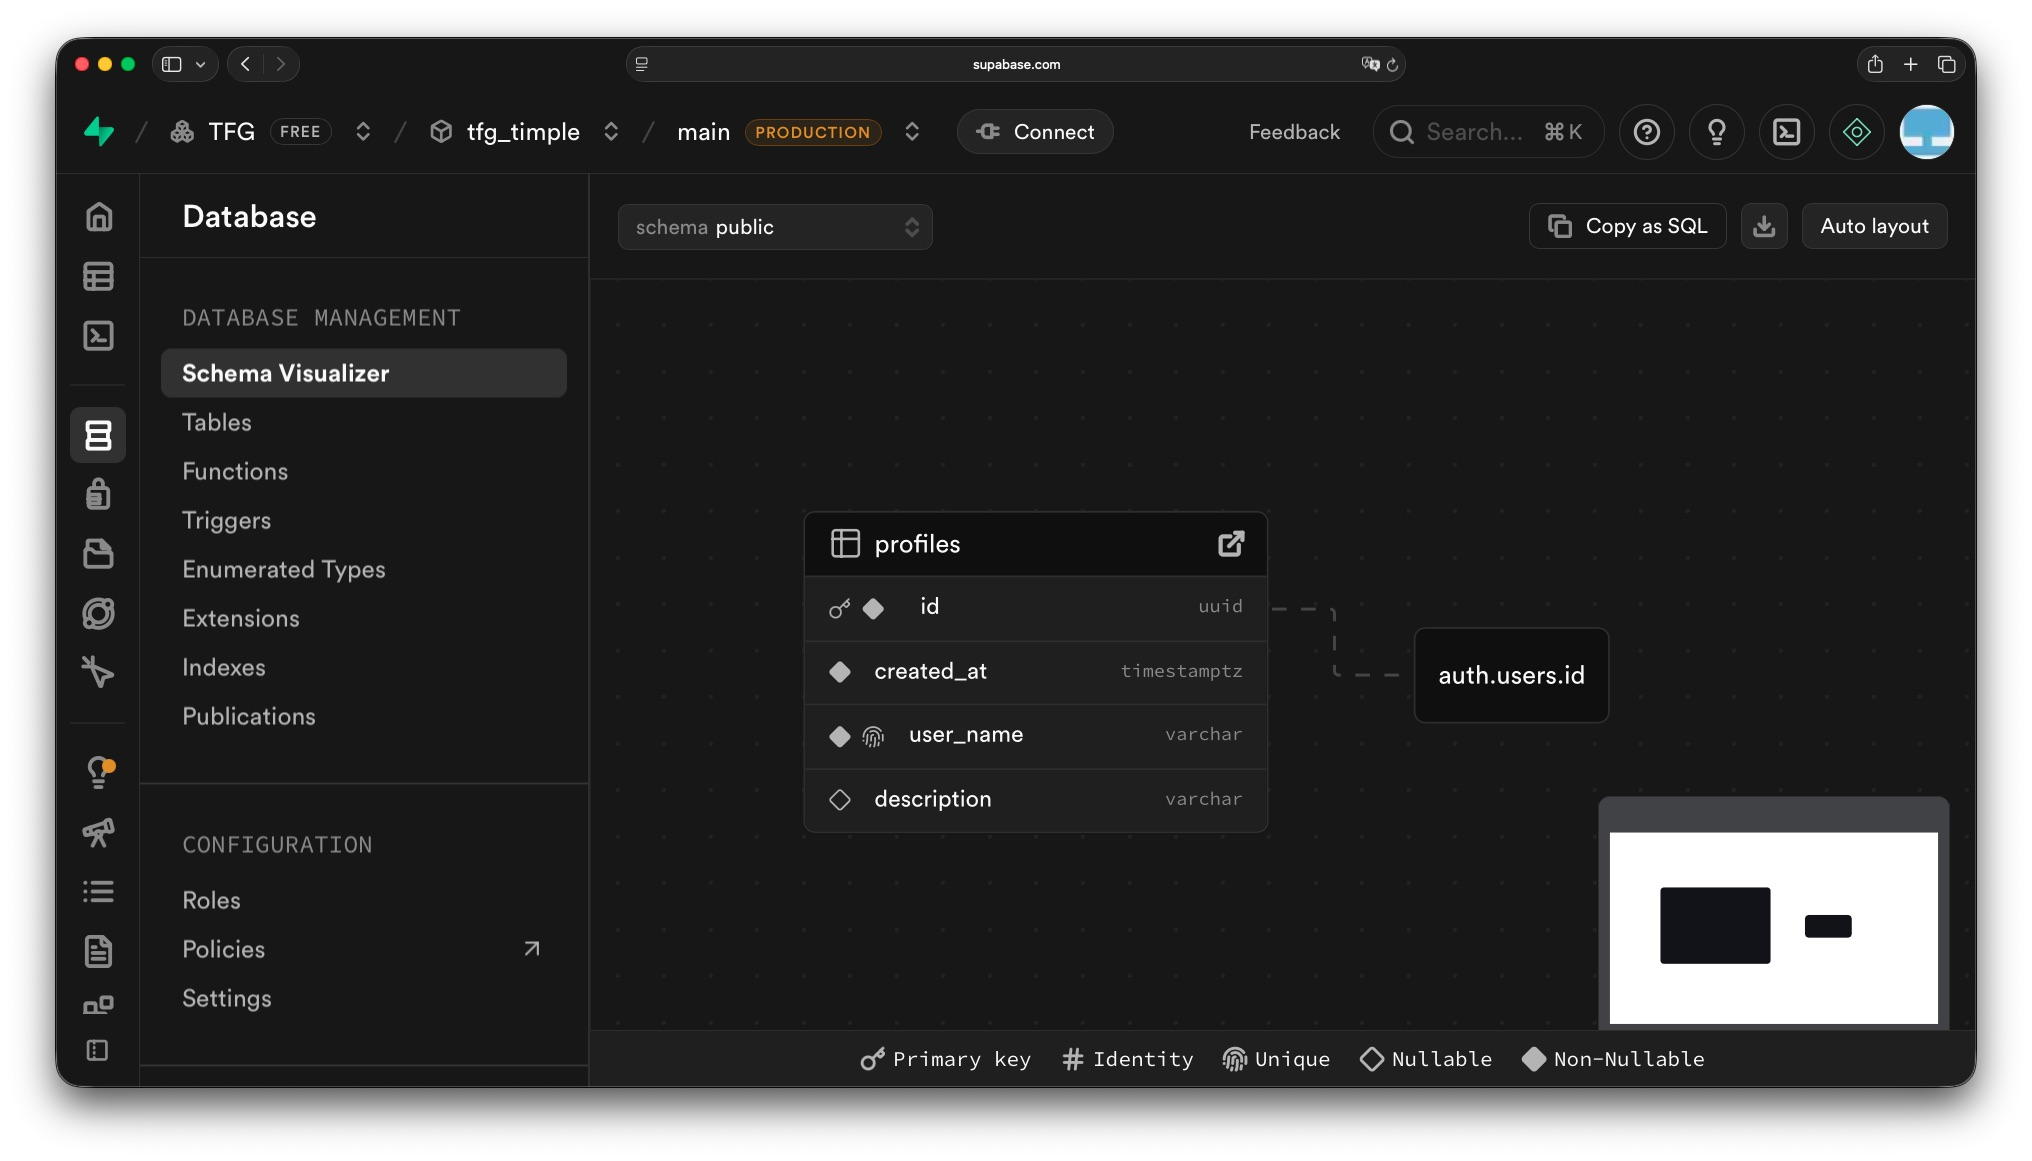
\includegraphics[width=\textwidth]{Ilustraciones/desarrollo/incremento1/desarrollo/supabase_profiles_table.jpeg}
        \caption{Tabla \textit{profiles} en \textit{Supabase}}\label{fig:supabase_profiles_table}
    \end{subfigure}\hfill
    \begin{subfigure}[t]{0.48\textwidth}
        \centering
        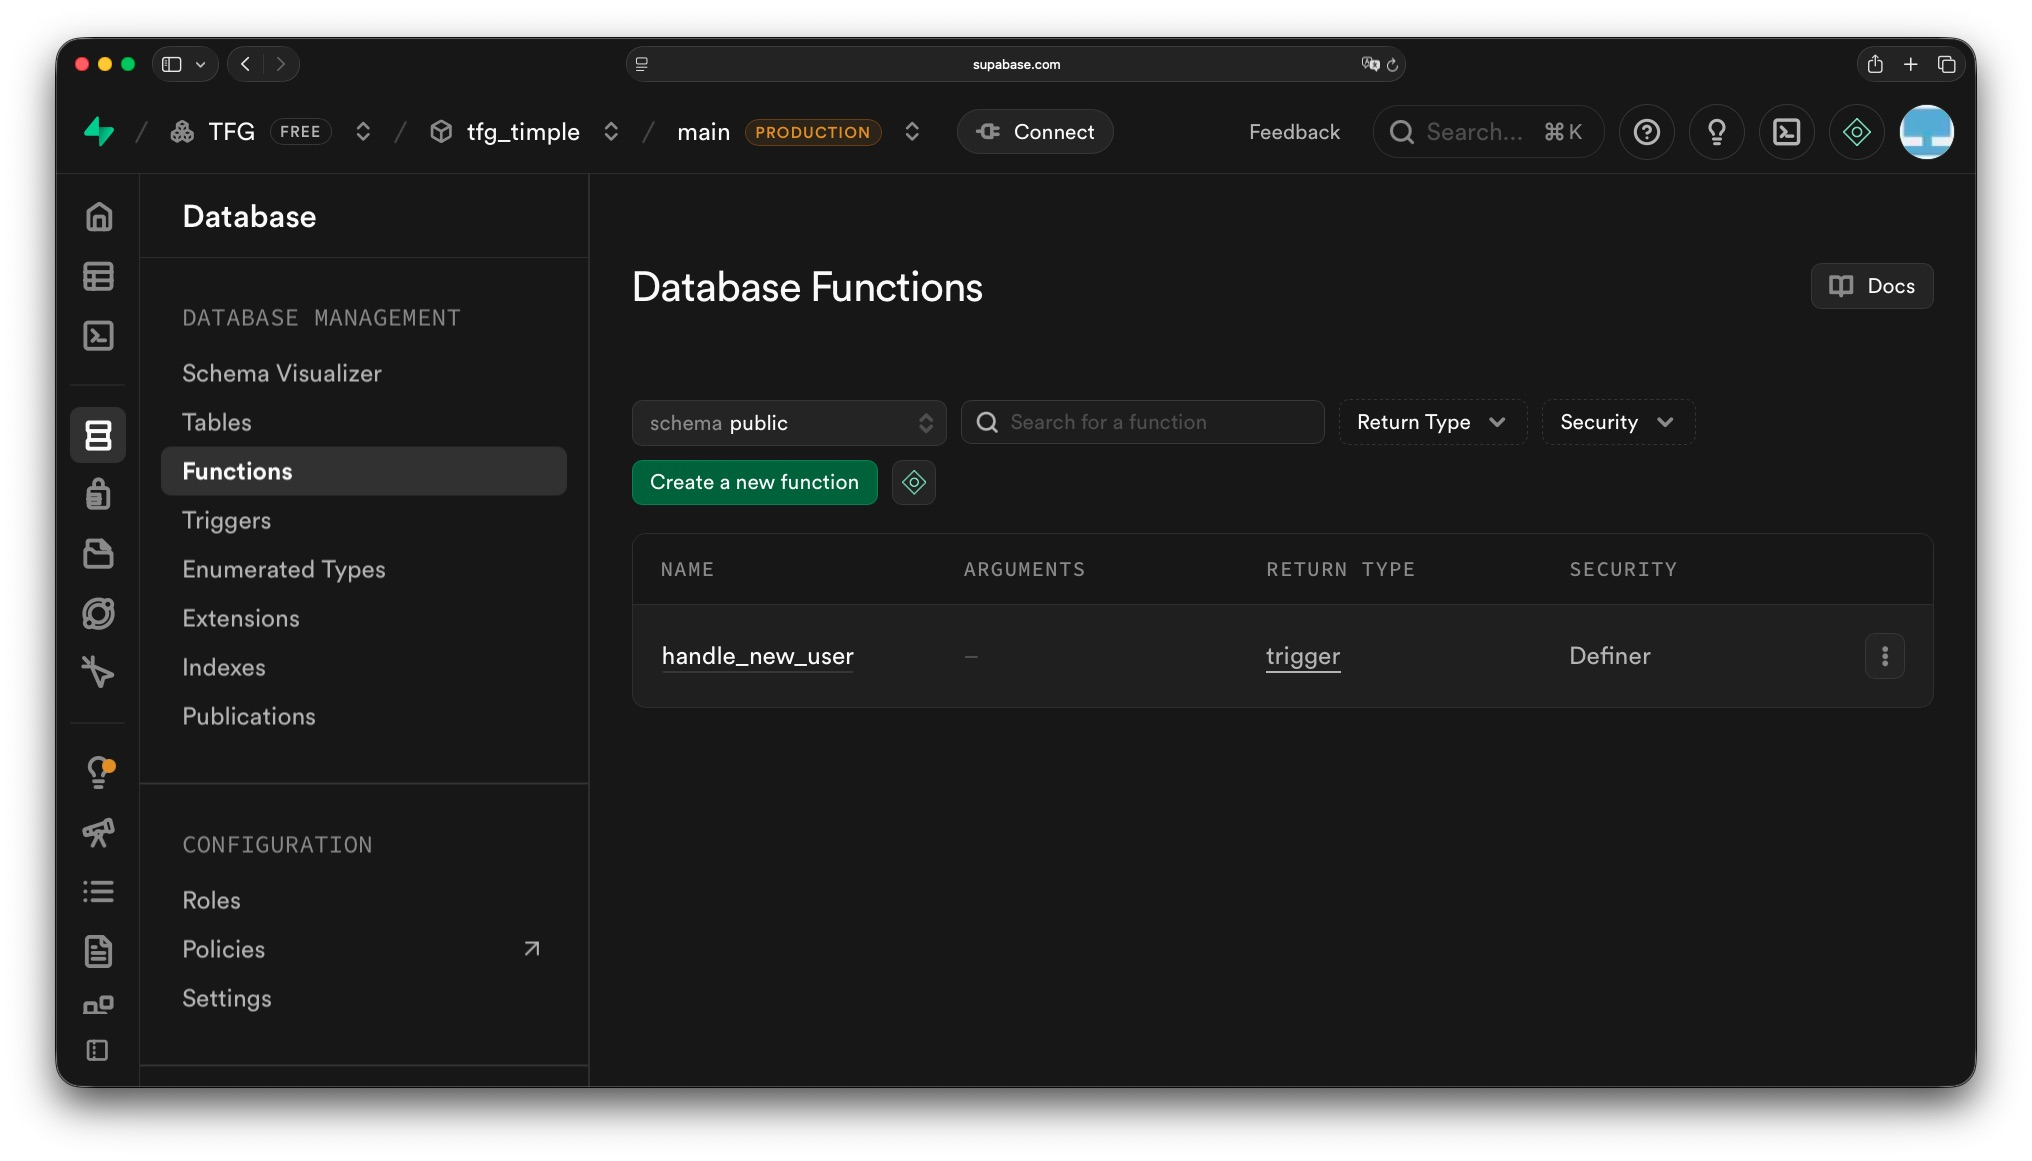
\includegraphics[width=\textwidth]{Ilustraciones/desarrollo/incremento1/desarrollo/supabase_username_function.jpeg}
        \caption{Función para la captación de nombre de usuario en los metadatos}\label{fig:supabase_username_function}
    \end{subfigure}
    \vspace{1em}

    \begin{subfigure}[t]{0.48\textwidth}
        \centering
        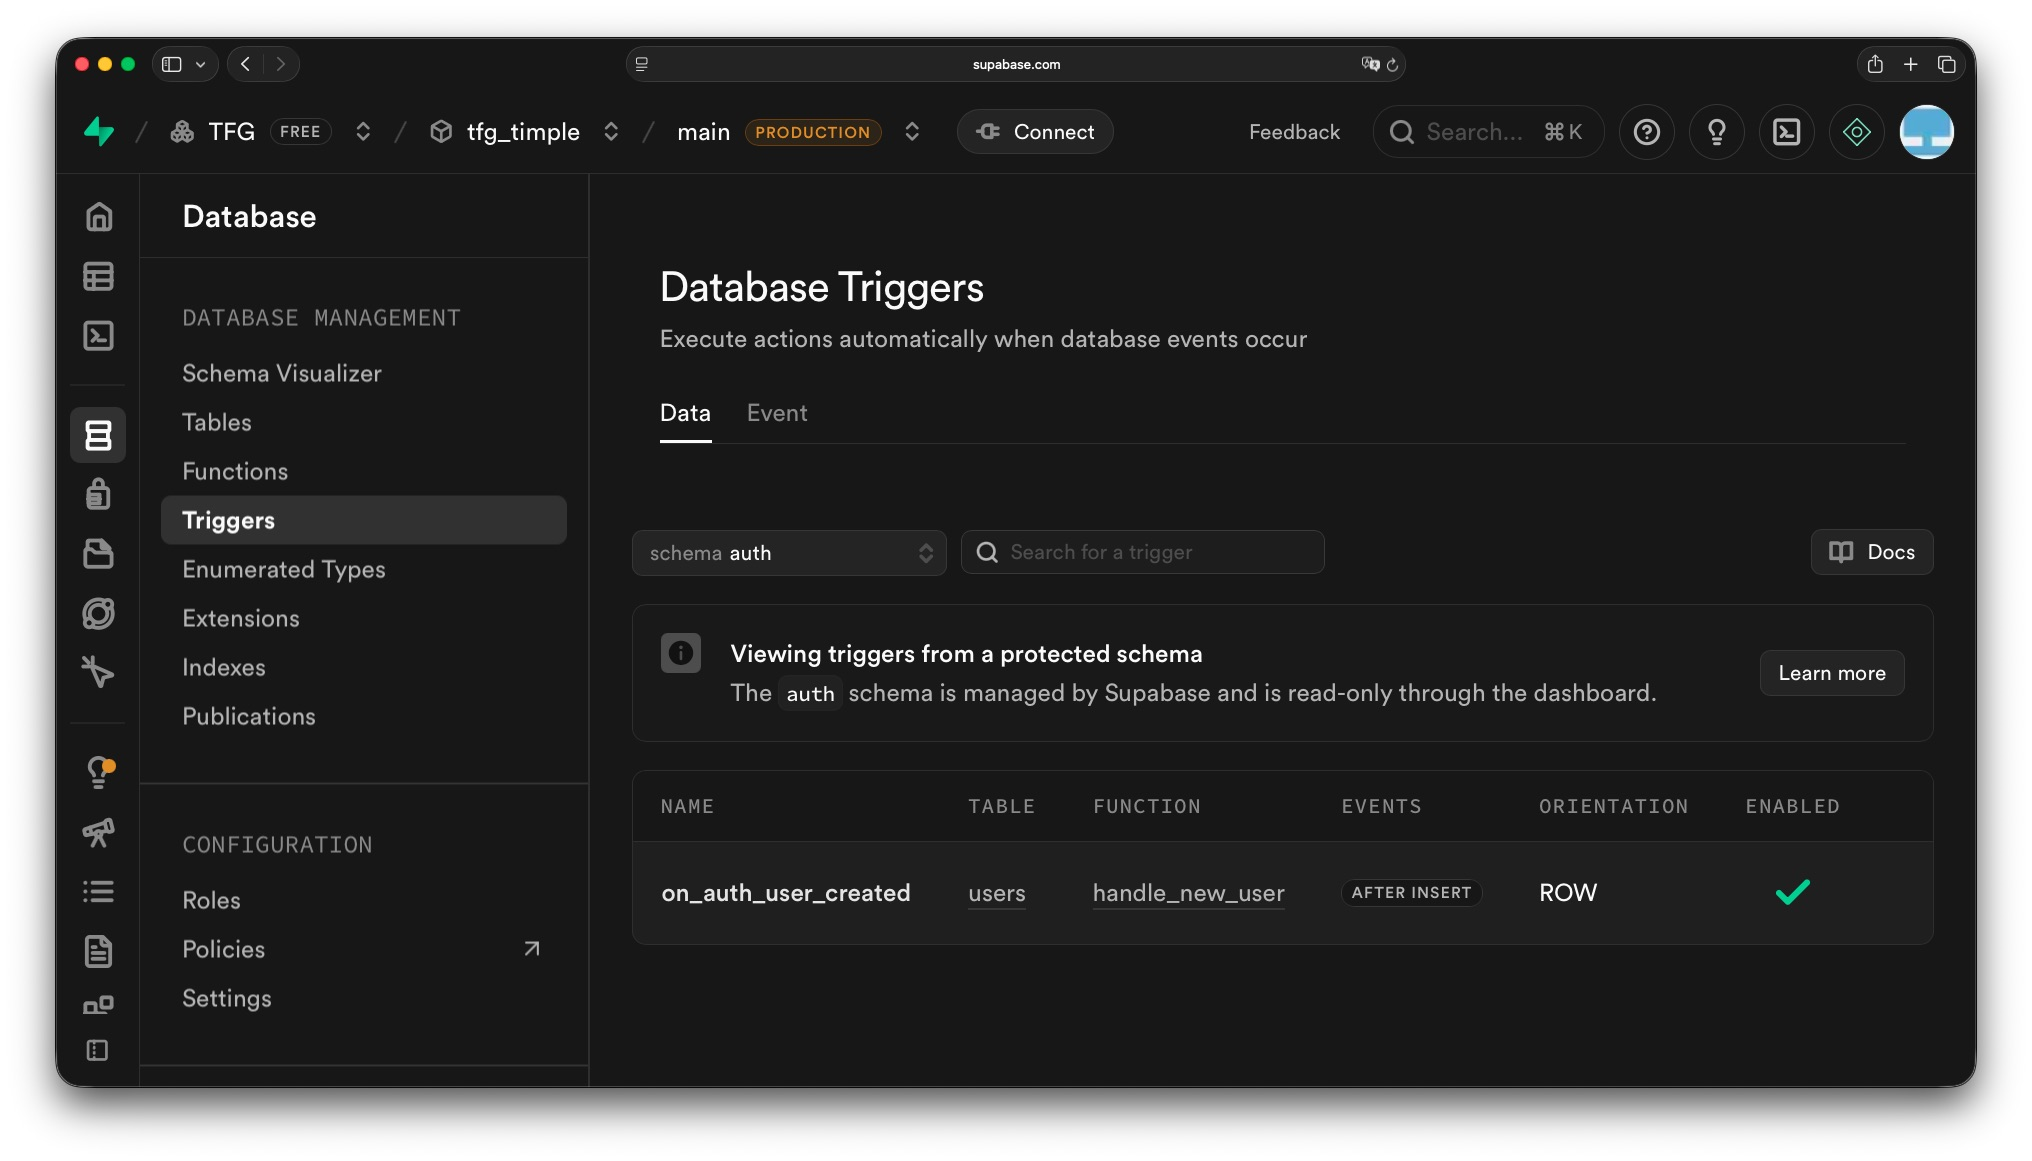
\includegraphics[width=\textwidth]{Ilustraciones/desarrollo/incremento1/desarrollo/supabase_username_trigger.jpeg}
        \caption{\textit{Trigger} con actuación tras el registro de usuario y ejecución de función de captación de nombre de usuario}\label{fig:supabase_username_trigger}
    \end{subfigure}\hfill
    \begin{subfigure}[t]{0.48\textwidth}
        \centering
        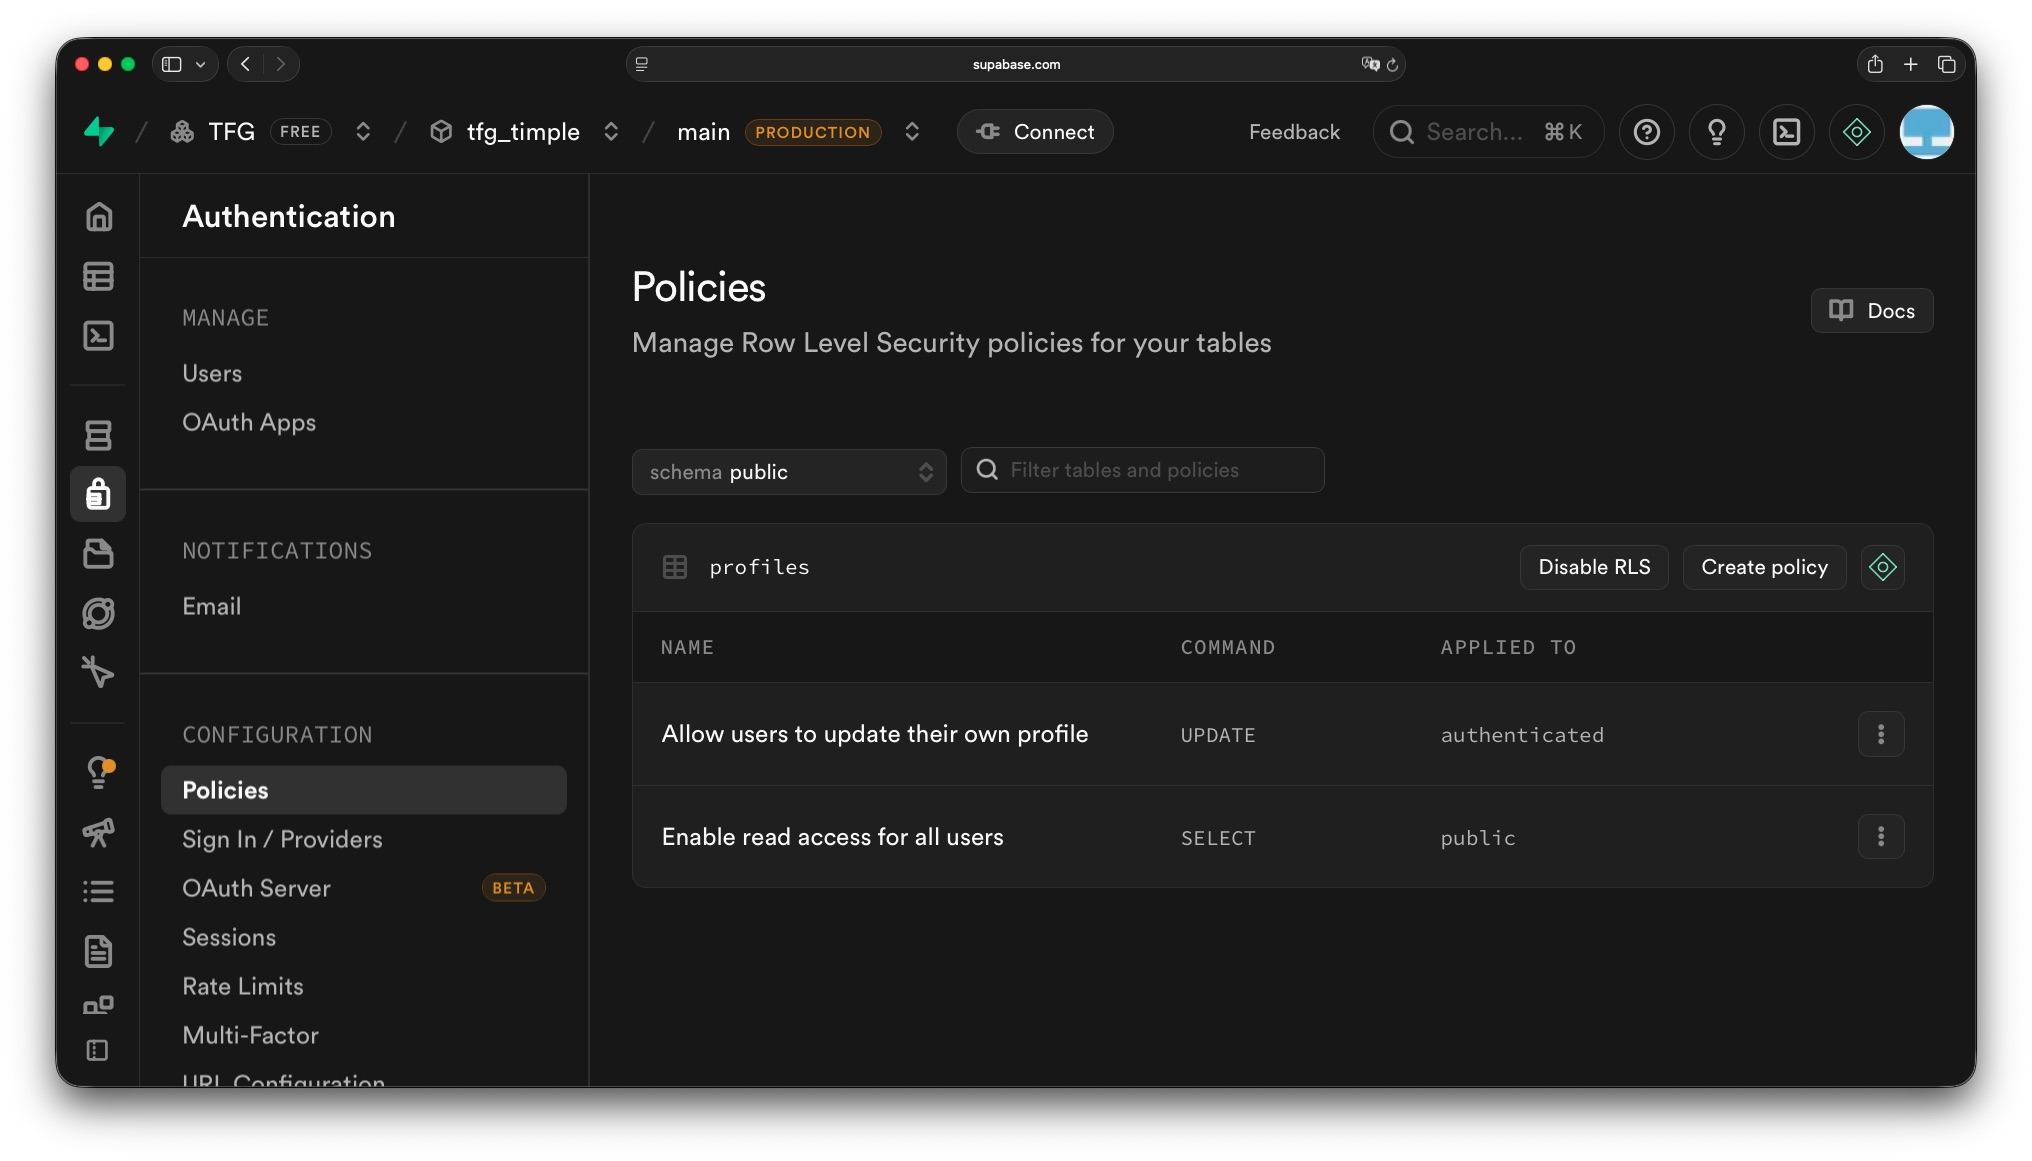
\includegraphics[width=\textwidth]{Ilustraciones/desarrollo/incremento1/desarrollo/supabase_policies.jpeg}
        \caption{Permisos de actualización y visualización de datos de la tabla \textit{public.profiles}}\label{fig:supabase_profiles_permissions}
    \end{subfigure}

    \caption{Creación de tabla \textit{public.profiles} y configuración de acciones y permisos}\label{fig:supabase_incremento_1}
\end{figure}

\textbf{En segundo lugar}, se creó un proyecto \textbf{Next.js} utilizando la plantilla \textbf{\textit{Next.js Supabase Auth Starter}}. Esta plantilla incluye:

\begin{itemize}
    \item \textbf{\textit{Middleware}} para el manejo de sesiones y acceso a páginas de usuarios autenticados y no autenticados.
    \item \textbf{Estilos preconfigurados} con paleta de colores predefinida.
    \item \textbf{Páginas de autenticación} para el registro, recuperación, inicio de sesión y errores.
    \item \textbf{Páginas con protección} con acceso limitado a usuarios autenticados.
    \item \textbf{Componentes} especialmente destinados a la ampliación y abstracción de etiquetas \textit{input}.
\end{itemize}

Además, se introdujeron las credenciales del proyecto creado en \textit{Supabase}, permitiendo la conexión de la plataforma con la plantilla.

\begin{figure}[H]
    \centering
    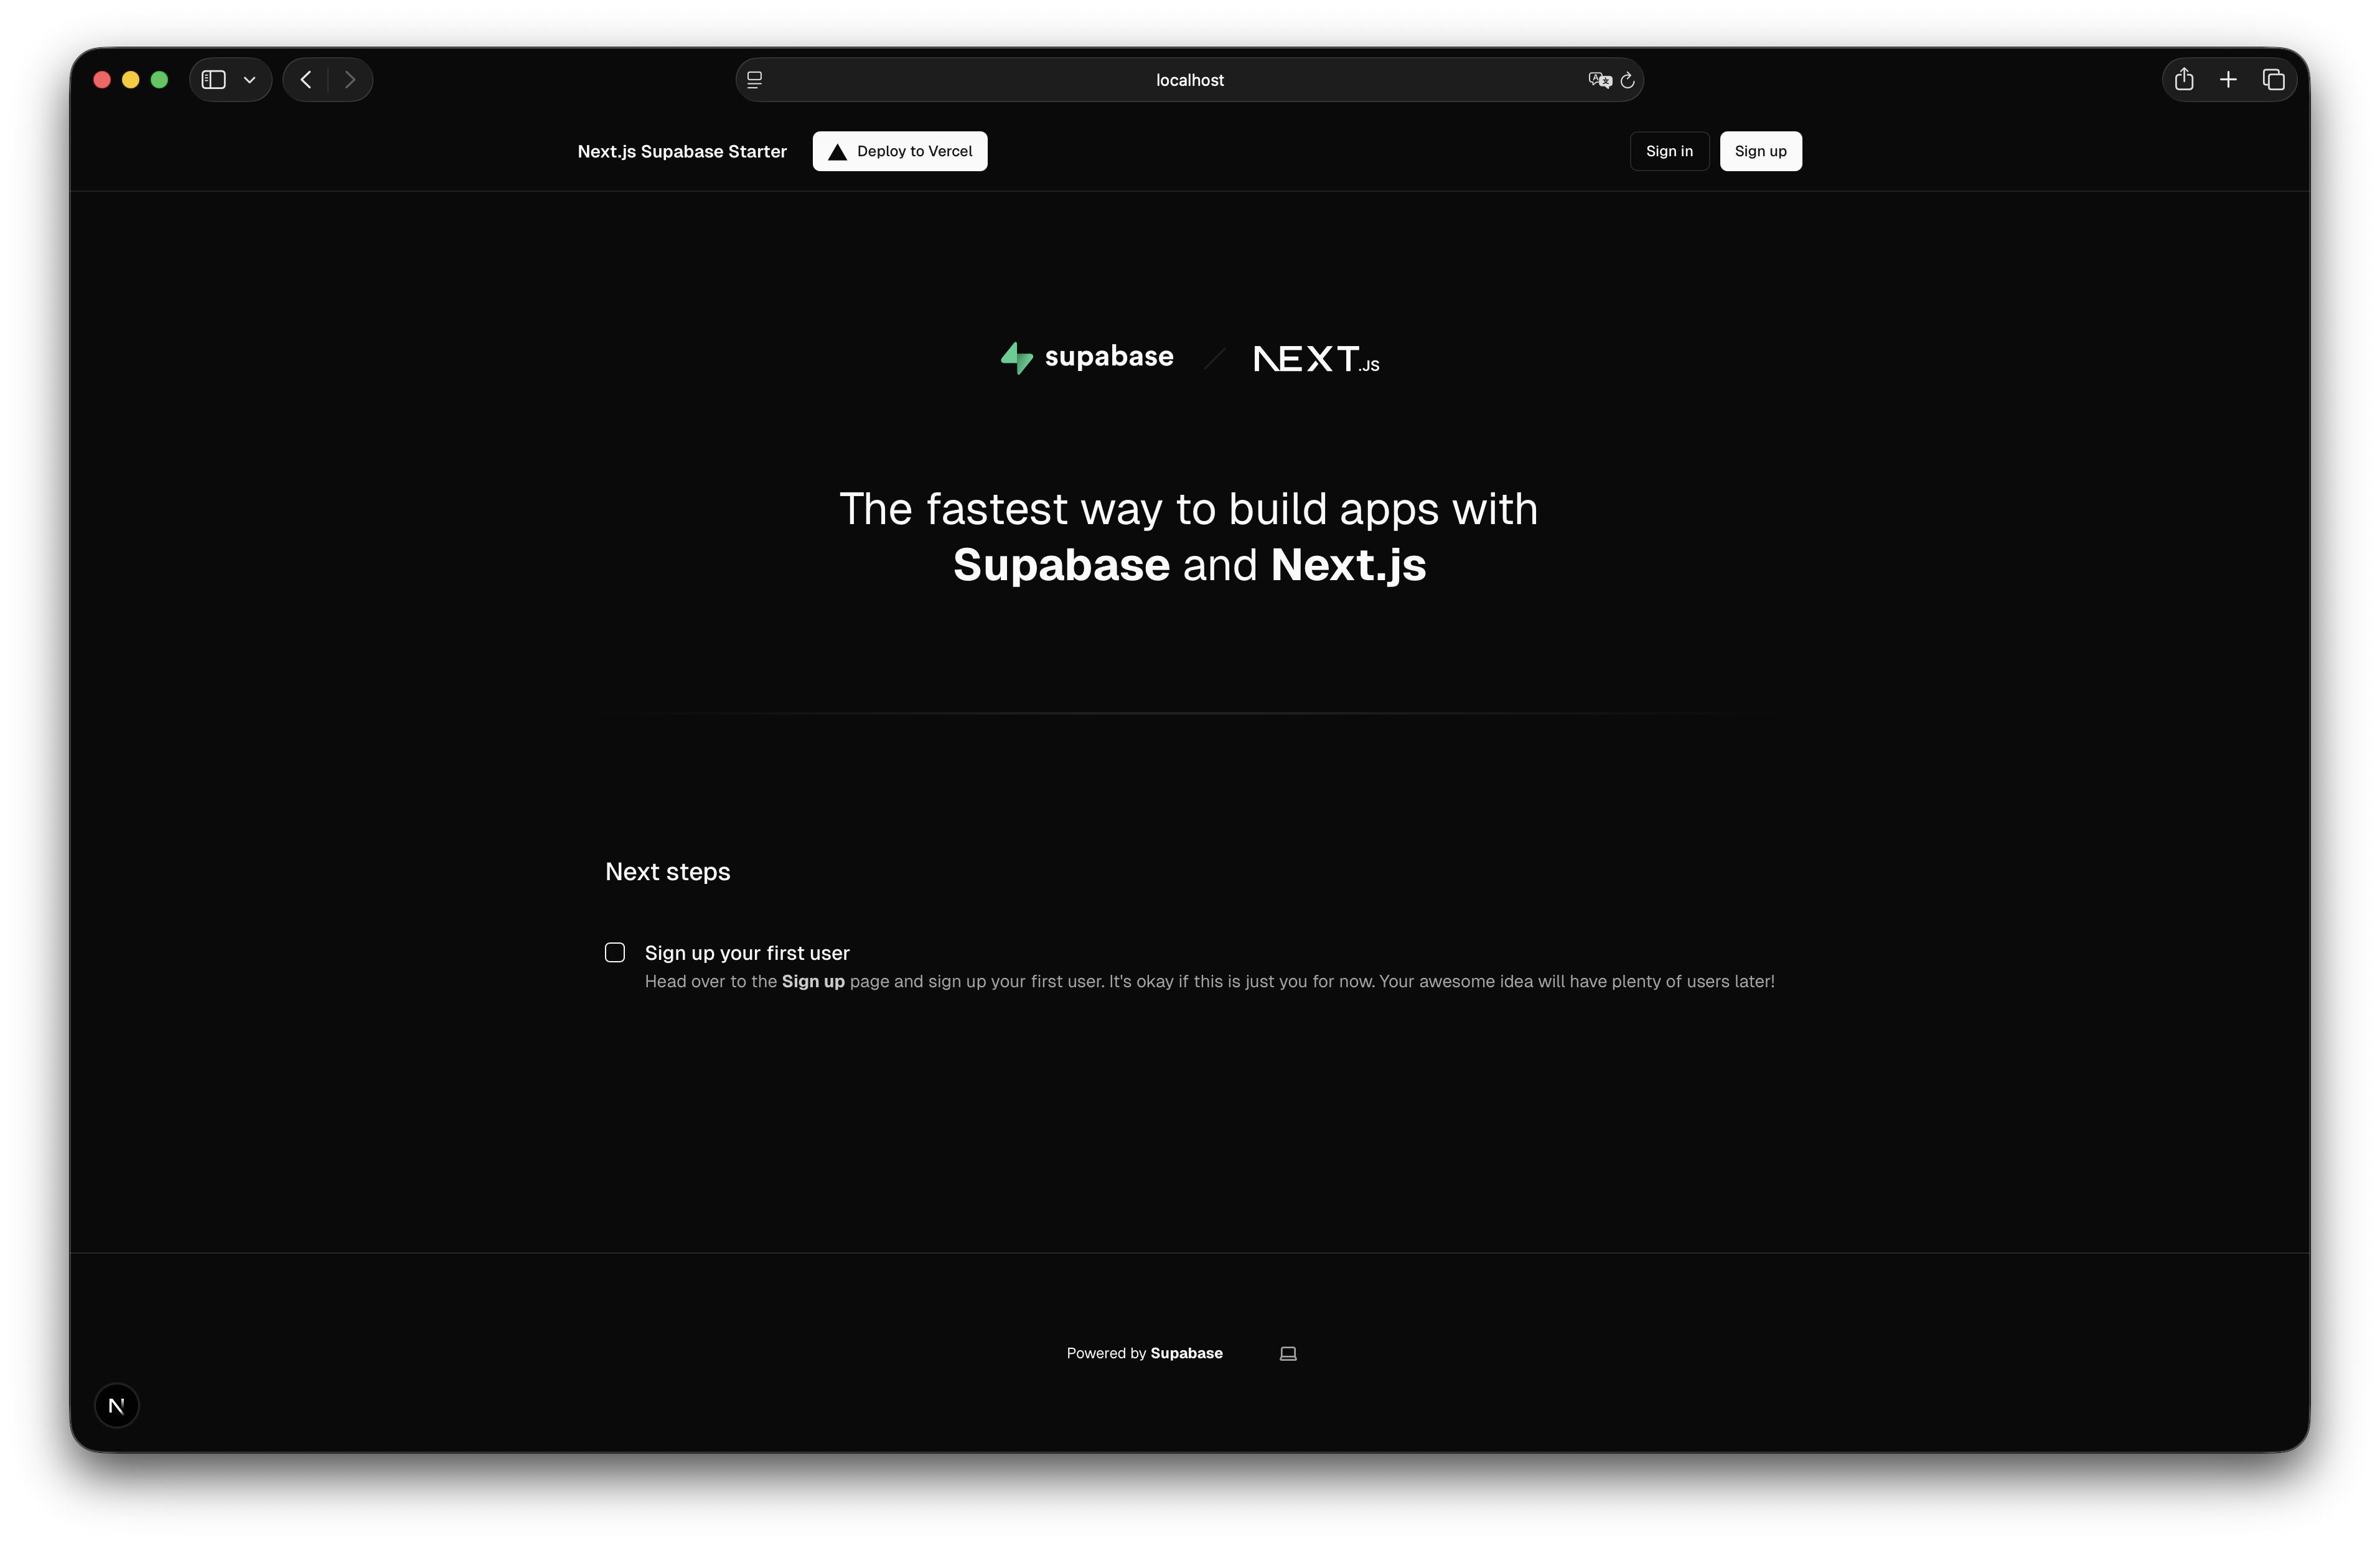
\includegraphics[width=0.8\textwidth]{Ilustraciones/desarrollo/incremento1/desarrollo/supabase_template.jpeg}    

    \caption{Plantilla de \textit{Next.js Supabase Auth Starter}}\label{fig:supabase_template}
\end{figure}

\textbf{En tercer lugar}, se realizó la actualización visual \figref{fig:login_1} adaptando la plantilla al diseño establecido en \capref{c:diseño_interfaz}.

\begin{figure}[H]
    \centering
    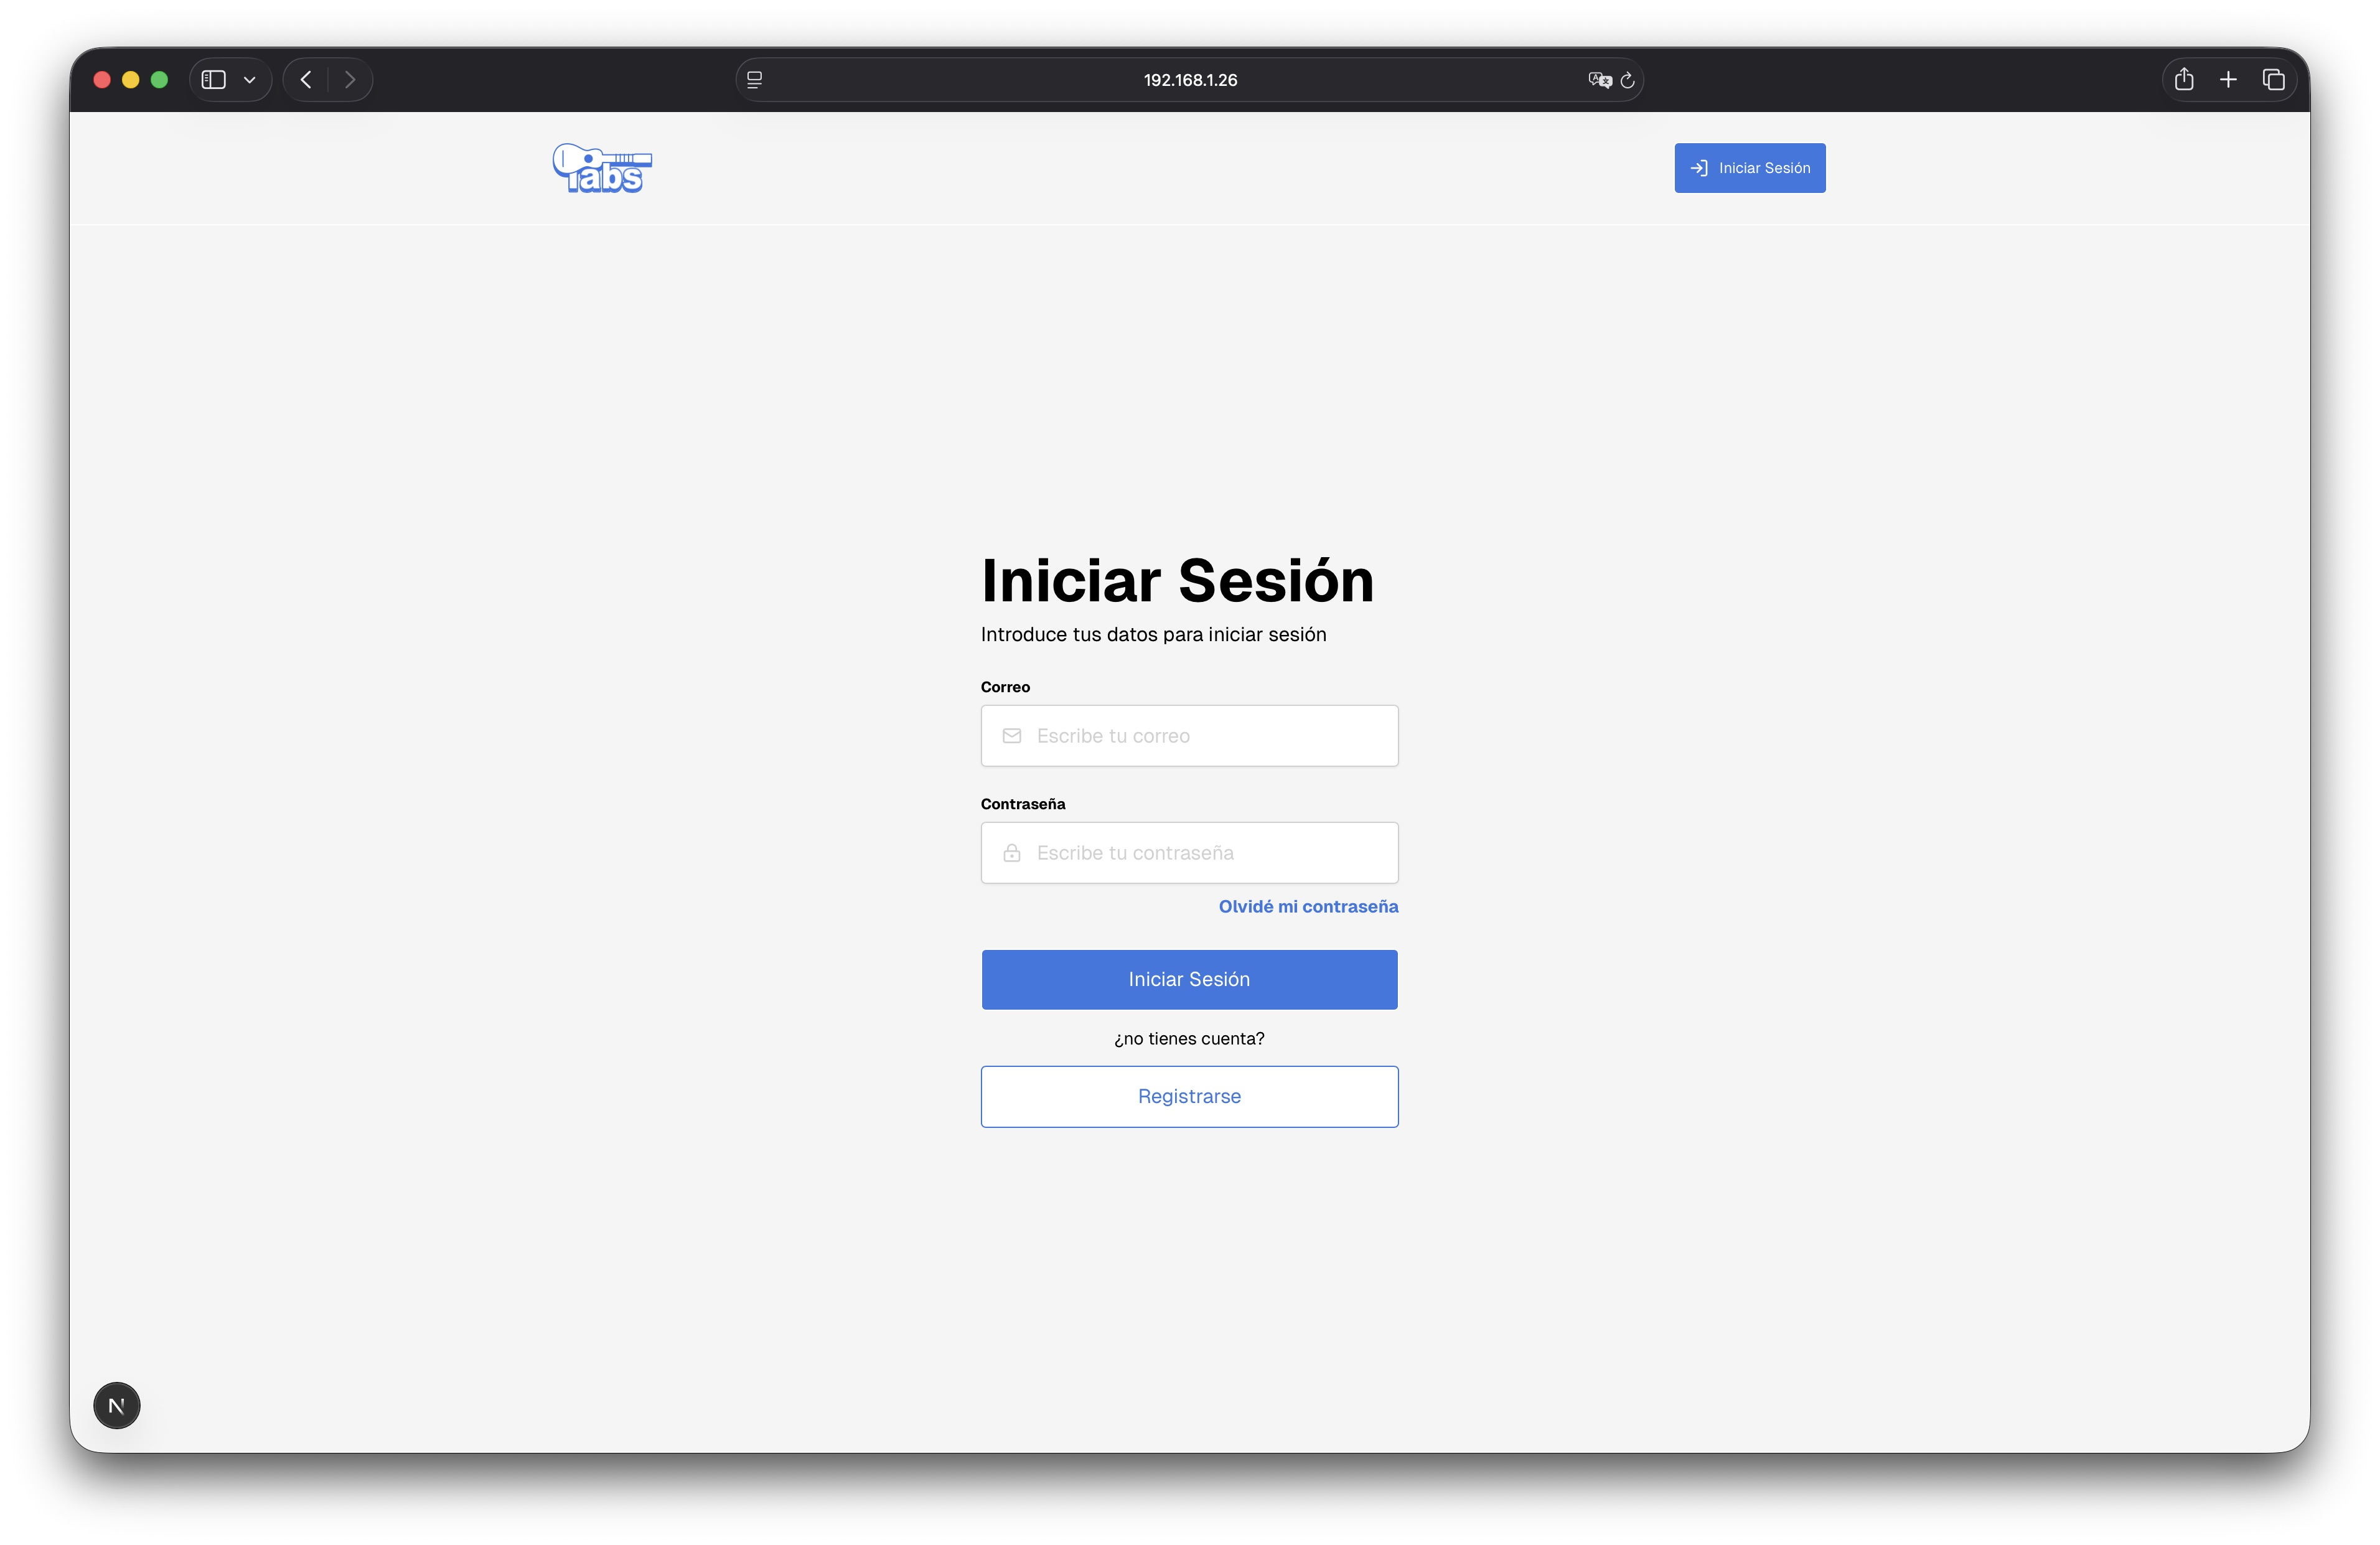
\includegraphics[width=0.8\textwidth]{Ilustraciones/desarrollo/incremento1/desarrollo/login_1.jpeg}    
    \caption{Plantilla de \textit{Next.js Supabase Auth Starter} con diseño actualizado}\label{fig:login_1}
\end{figure}

\textbf{En cuarto lugar}, se realizaron cambios en cuanto a la organización de directorios y la modularización de funciones existentes en componentes del lado del cliente:

\begin{enumerate}
    \item Se implementó la siguiente organización de directorios \figref{fig:directory_order}:
        \begin{itemize}
            \item \textbf{\textit{/app}}, donde se encuentran las páginas de acceso público y privado.
            \item \textbf{\textit{/components}}, donde se agrupan los componentes del lado del cliente, distinguiendo dos subdirectorios: \textit{/ui}, destinado a los elementos comunes de la interfaz \textit{(i.e., botones, campos, diálogos, etc.)}, y otros componentes diseñados para modularizar y abstraer secciones de código de las páginas.
            \item \textbf{\textit{/lib}}, que contiene la lógica de negocio del proyecto:
                \begin{itemize}
                    \item \textbf{\textit{/actions}}, donde se localizan los validadores \textit{(i.e., tamaño de contraseña, longitud de descripción, existencia de nombre de usuario, etc.)}.
                    \item \textbf{\textit{/domains}}, que alberga los componentes del lado del servidor responsables de la ejecución de consultas a \textit{Supabase}.
                    \item \textbf{\textit{/dto}}, donde se definen las interfaces correspondientes a los \textit{DTO}.
                    \item \textbf{\textit{/supabase}}, que contiene la configuración, las credenciales de acceso y el \textit{middleware} de \textit{Supabase}.
                    \item \textbf{\textit{/errors}}, donde se encuentran los identificadores de errores y sus mensajes asociados.
                    \item \textbf{\textit{/mappers}}, que incluye las funciones encargadas de la construcción de los \textit{DTO}.
                \end{itemize}
        \end{itemize}

    \begin{figure}[H]
        \centering
        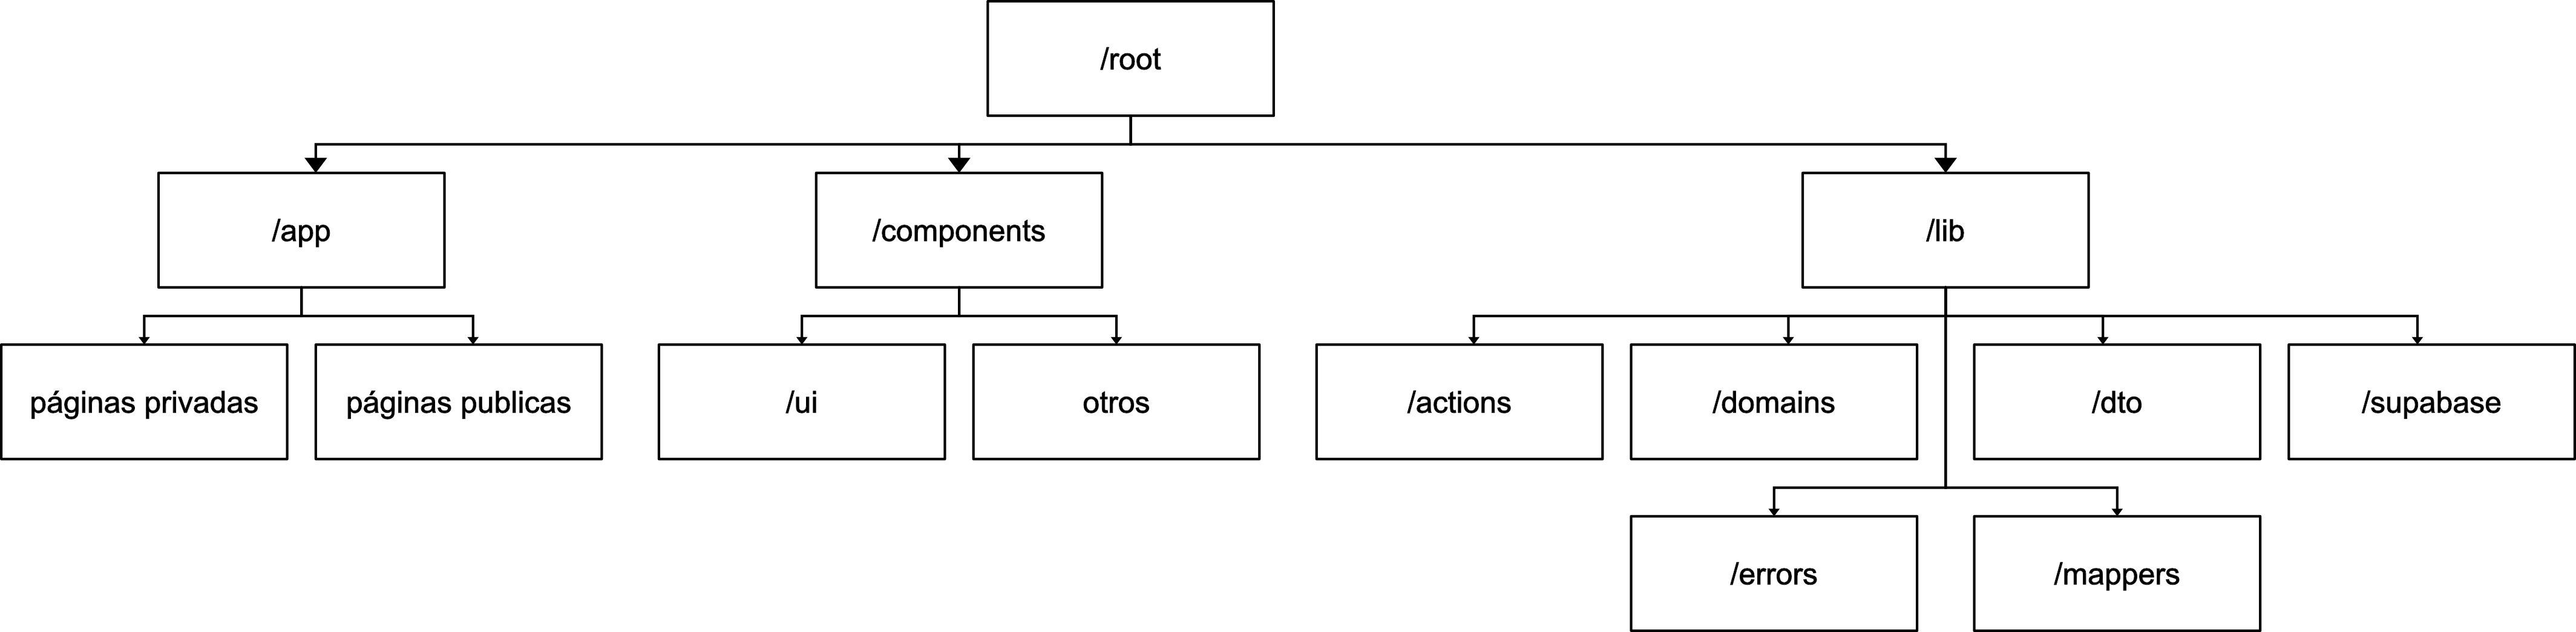
\includegraphics[width=1\textwidth]{Ilustraciones/desarrollo/incremento1/desarrollo/dir_ord.jpg}    
        \caption{Organización de directorios en el proyecto}
        \label{fig:directory_order}
    \end{figure}

    \item Se realizaron modificaciones sobre las páginas y componentes proporcionados por la plantilla, modularizando sus funciones de consulta a través de la implementación de \textit{DTO}, \textit{mappers}, validadores y componentes del lado del servidor.
\end{enumerate}

\textbf{En quinto lugar}, se procedió a la implementación de las páginas y componentes relacionados con los objetivos restantes a cubrir:

\begin{itemize}
    \item Las páginas de \textbf{manual del usuario} \figref{fig:manual} y \textbf{preguntas frecuentes}, donde se implementaron colecciones que almacenan toda la información a mostrar, facilitando la adición y modificación de contenidos.
    
    \begin{figure}[H]
        \centering
        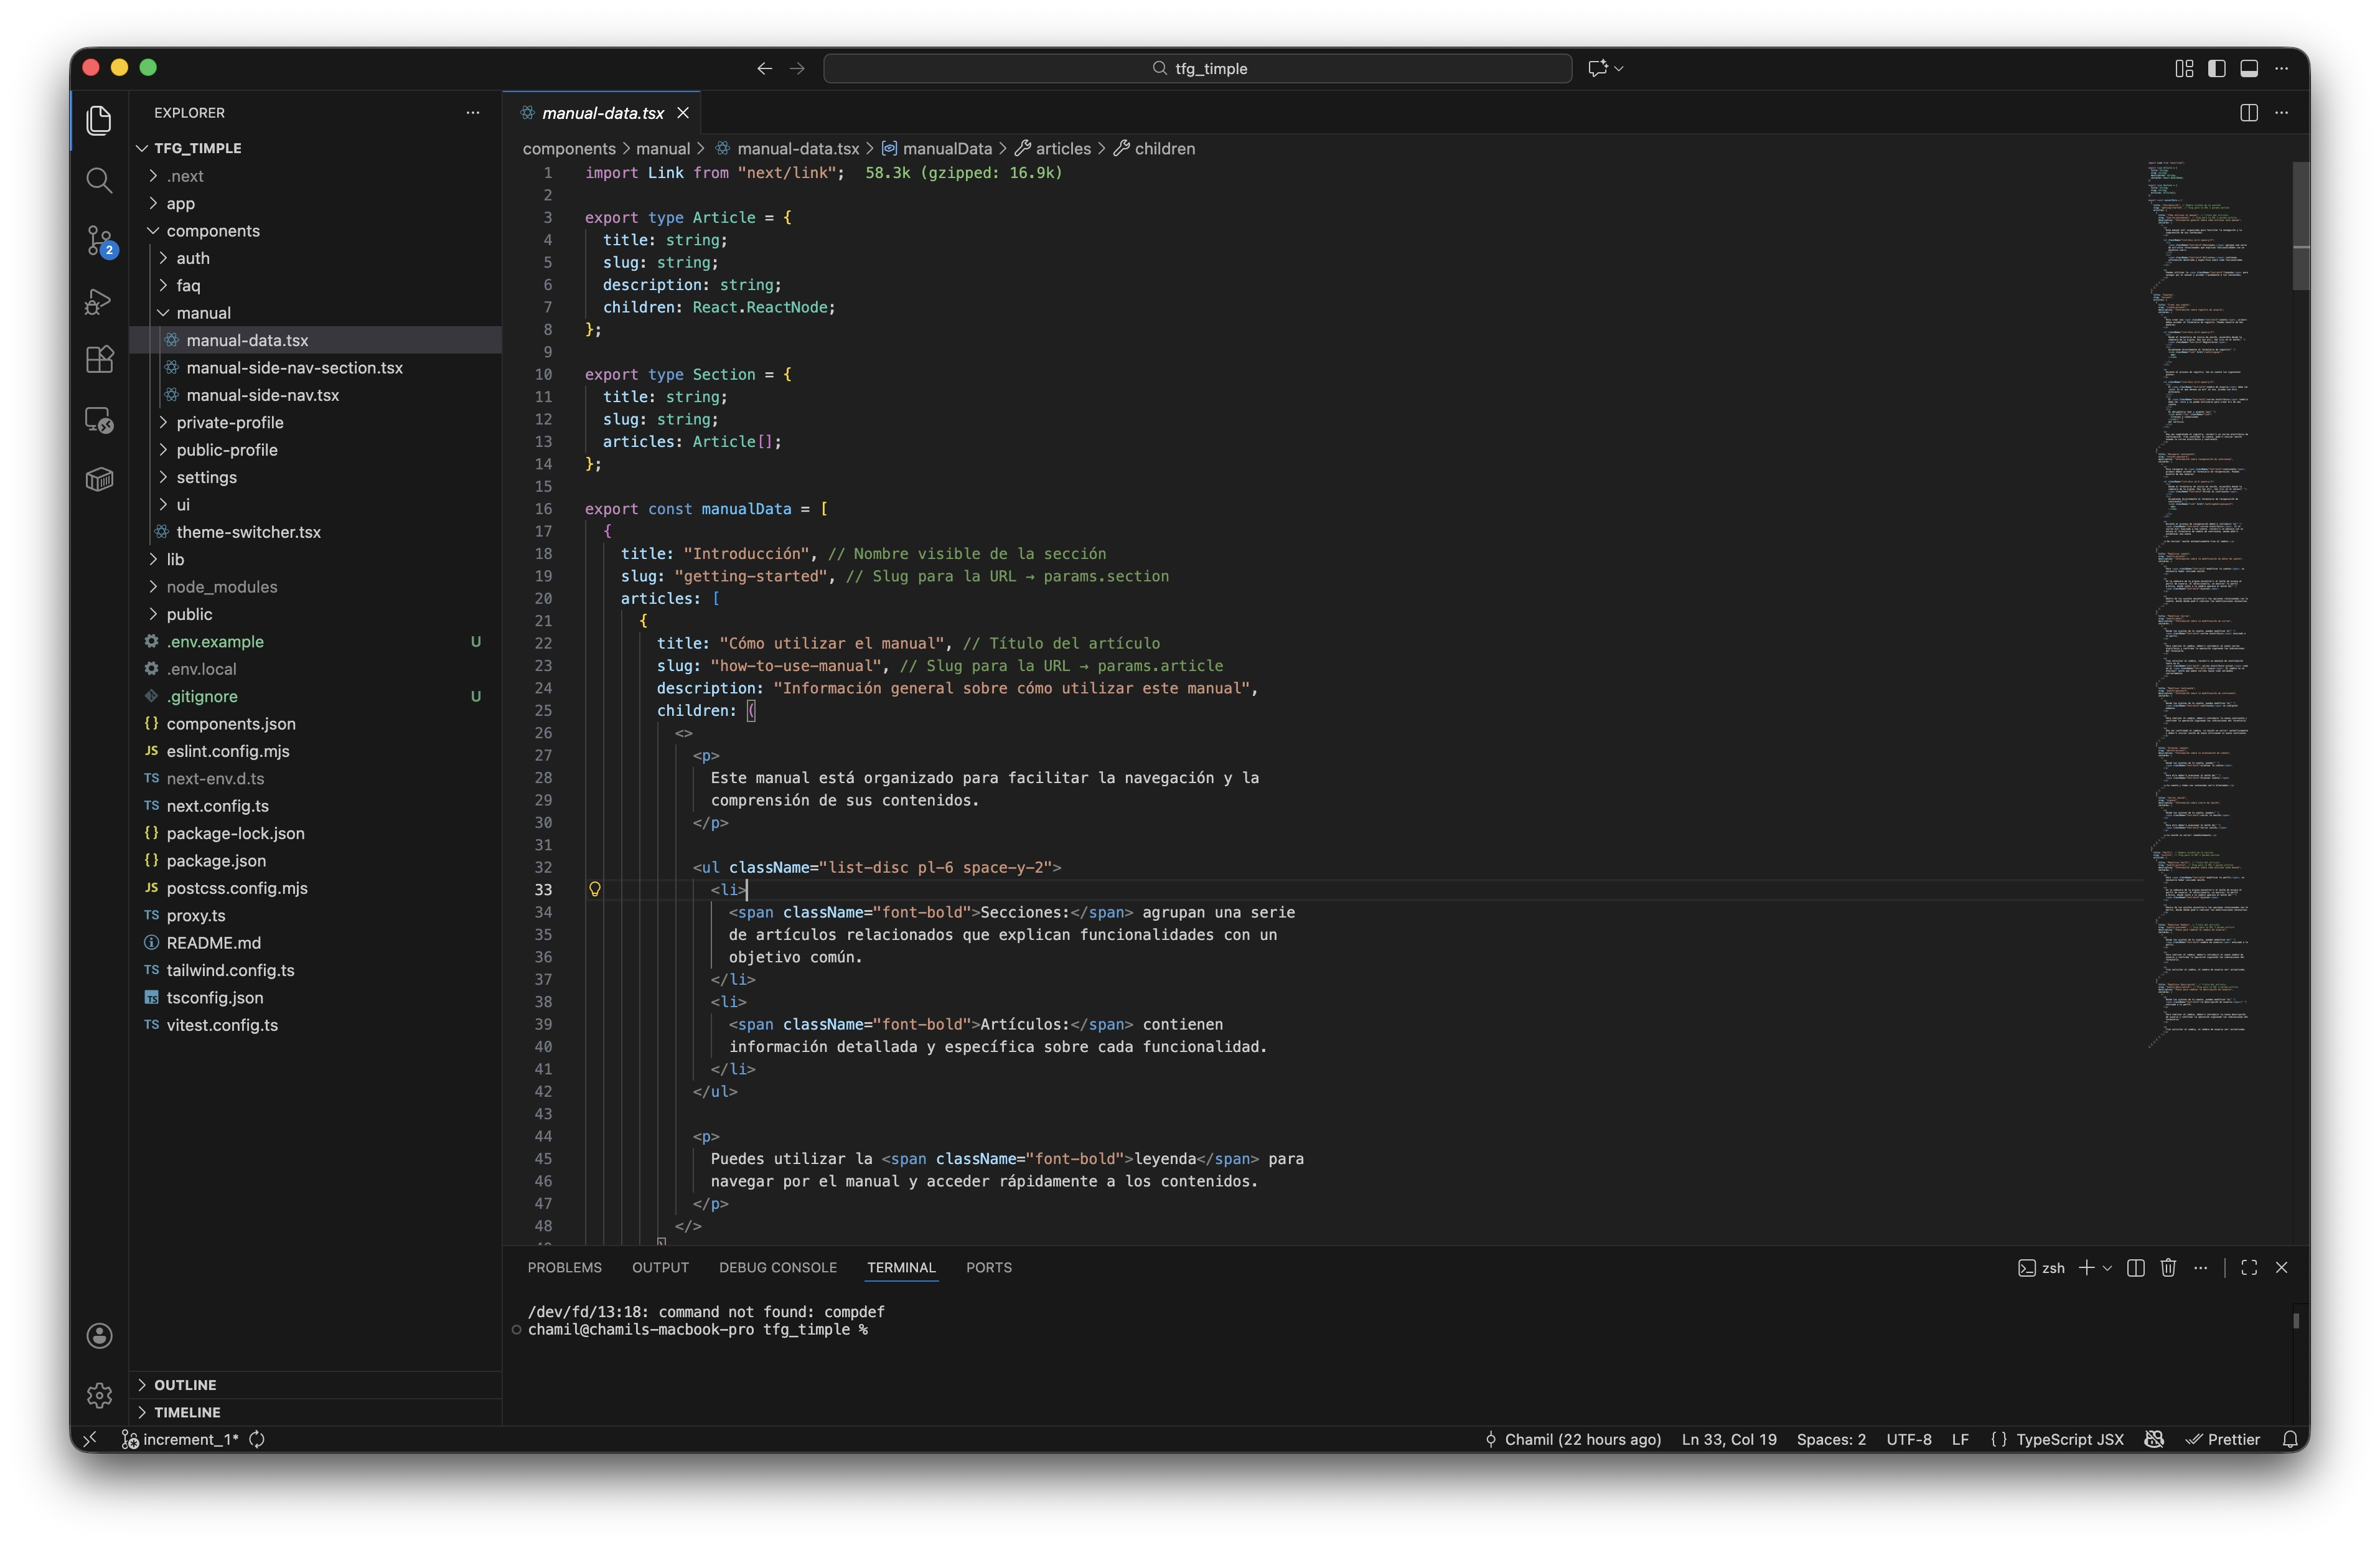
\includegraphics[width=0.8\textwidth]{Ilustraciones/desarrollo/incremento1/desarrollo/manual_it1.jpeg}
        \caption{Colección de información del manual de usuario}\label{fig:manual}
    \end{figure}

    \item Las páginas de \textbf{perfil público y privado de usuario} y \textbf{ajustes de cuenta}, donde se desarrollaron \textit{DTO}, \textit{mappers}, y componentes del lado del servidor adaptados a cada página.  Además, destaca la implementación de dialogos de varios pasos \figref{fig:dialogs}, estableciendo un proceso de advertencia, modificación y confirmación del resultado.
    
    \begin{figure}[H]
        \centering
        \begin{subfigure}[t]{0.31\textwidth}
            \centering
            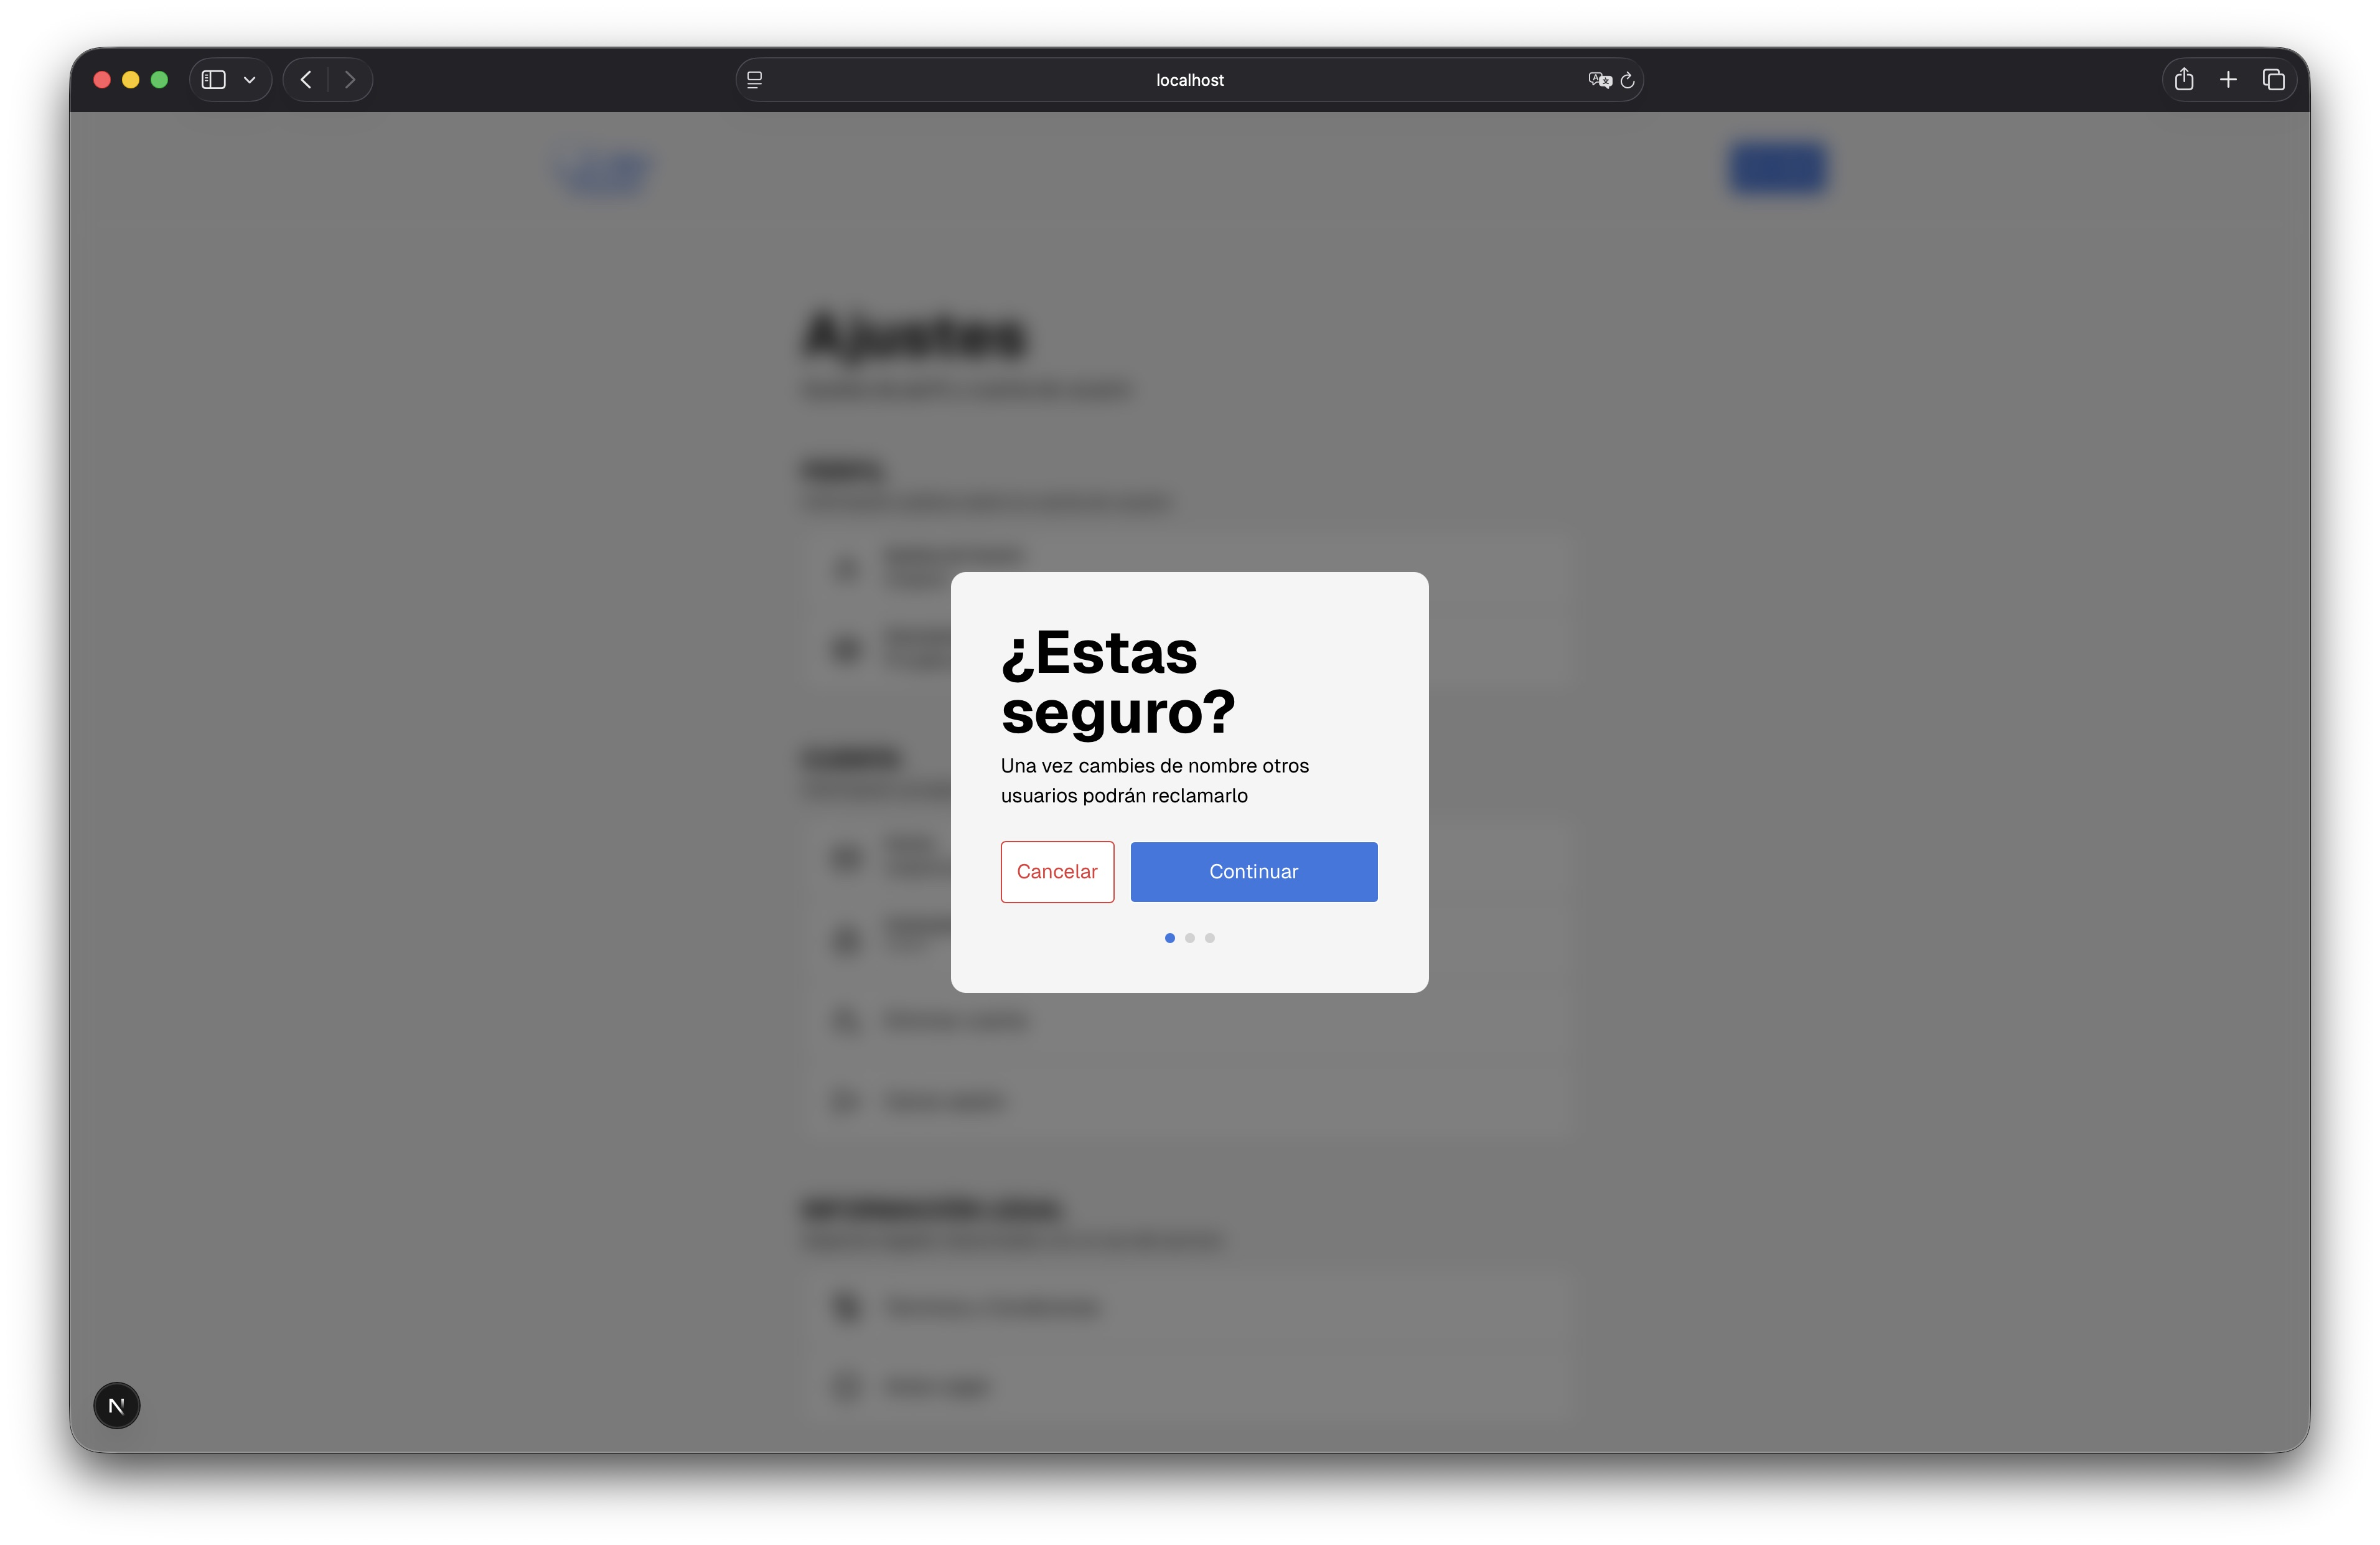
\includegraphics[width=\textwidth]{Ilustraciones/desarrollo/incremento1/desarrollo/dialog_1.jpeg}
            \caption{Dialogo de advertencia para la modificación de nombre de usuario}\label{fig:dialog_1}
        \end{subfigure}\hfill
        \begin{subfigure}[t]{0.31\textwidth}
            \centering
            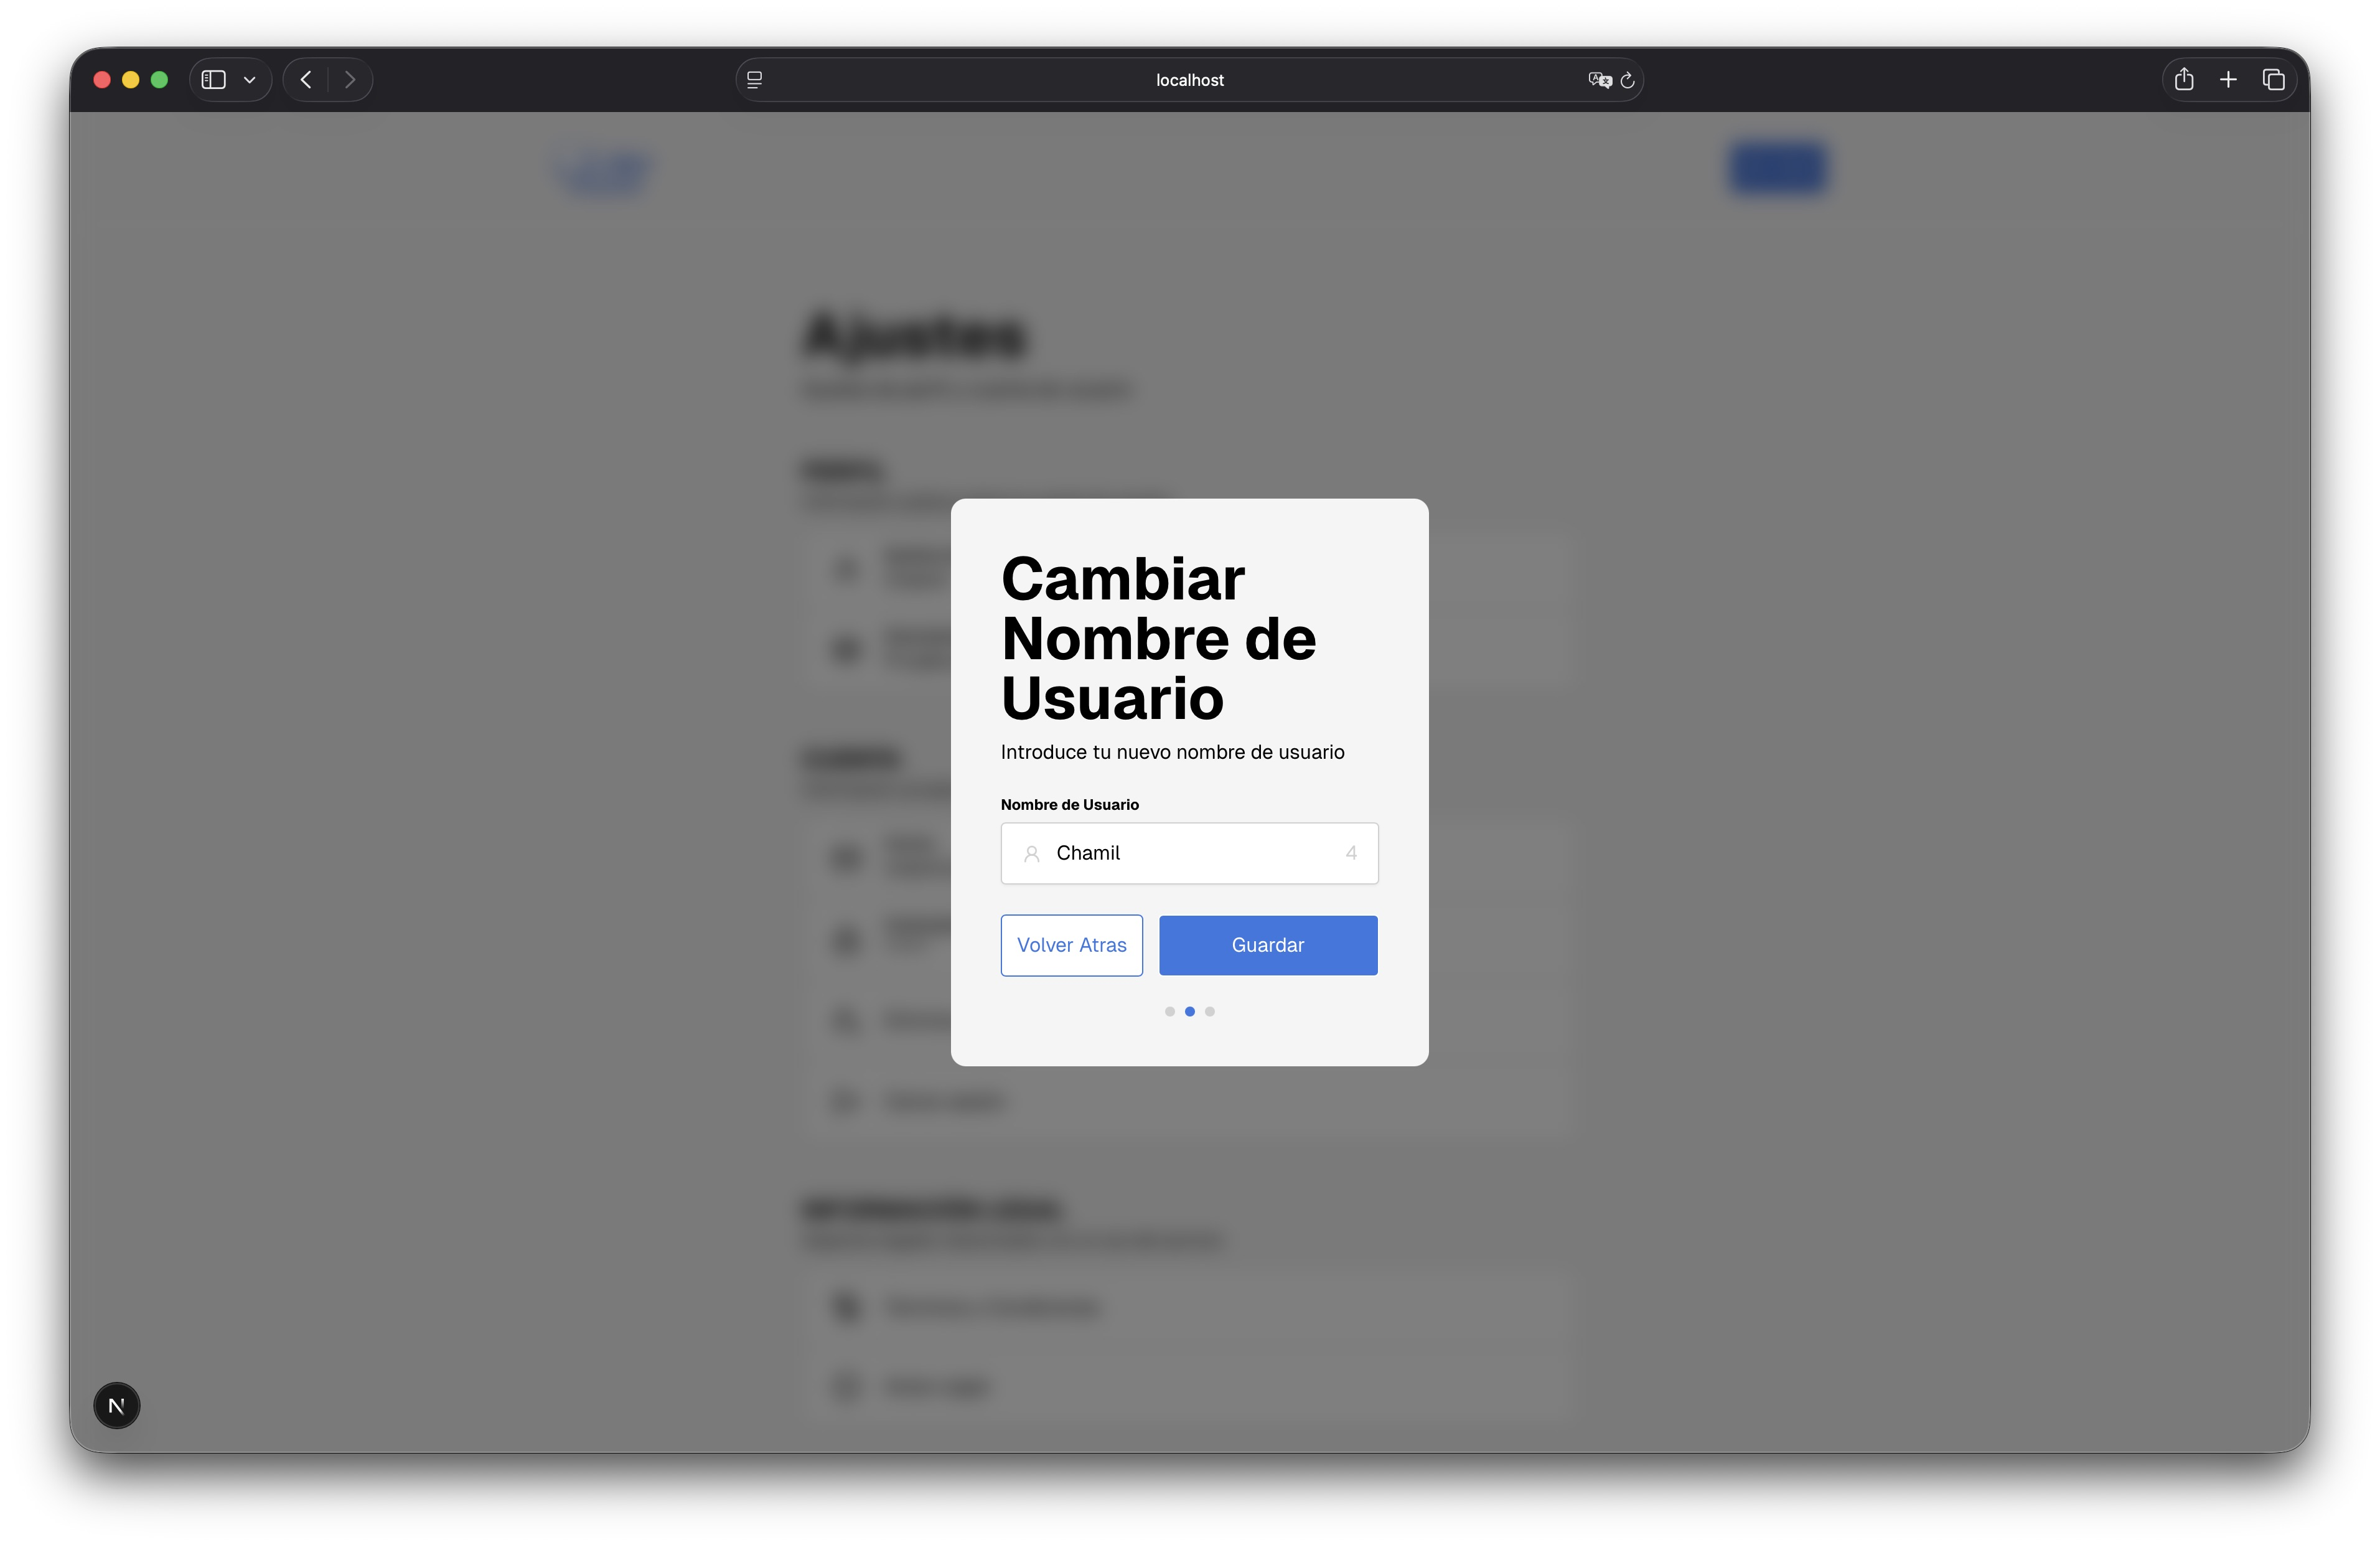
\includegraphics[width=\textwidth]{Ilustraciones/desarrollo/incremento1/desarrollo/dialog_2.jpeg}
            \caption{Dialogo de formulario para la modificacion de nombre de usuario}\label{fig:dialog_2}
        \end{subfigure}\hfill
        \begin{subfigure}[t]{0.31\textwidth}
            \centering
            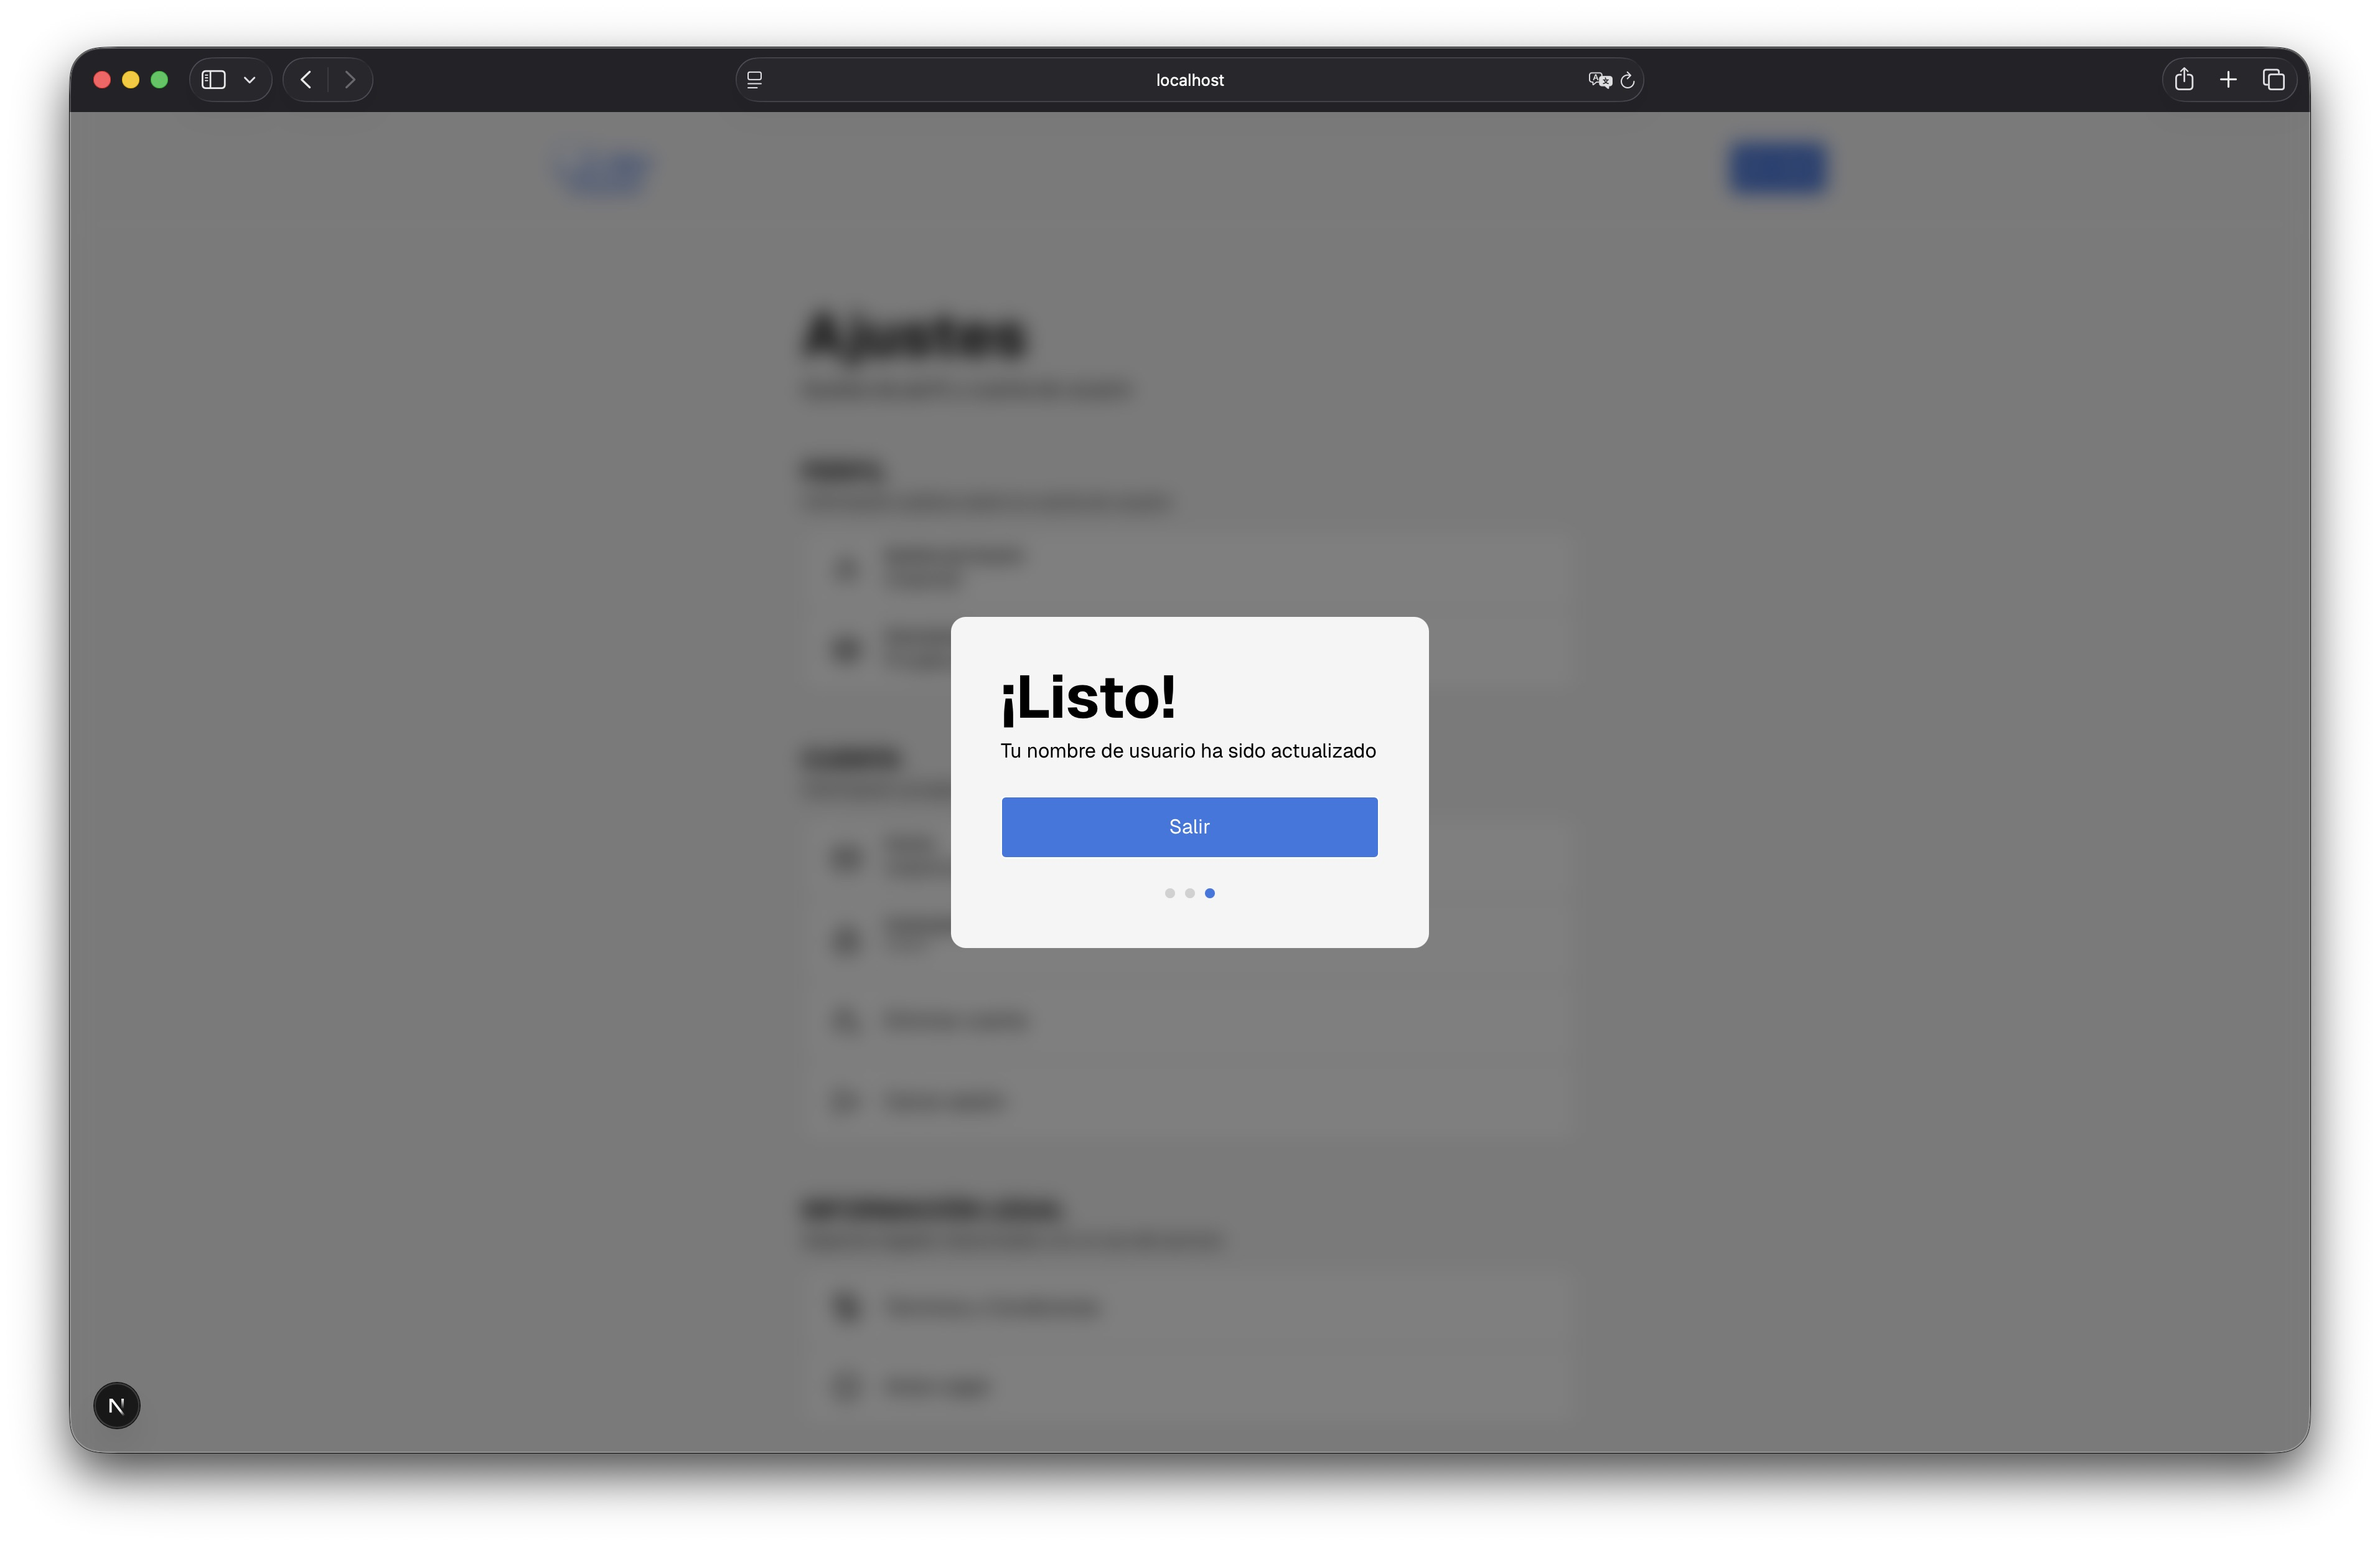
\includegraphics[width=\textwidth]{Ilustraciones/desarrollo/incremento1/desarrollo/dialog_3.jpeg}
            \caption{Dialogo de confirmación de cambio}\label{fig:dialog_3}
        \end{subfigure}
        
        
        \caption{Dialogos para la modificación de datos de cuenta}\label{fig:dialogs}
    \end{figure}

    \item Las páginas de \textbf{aviso legal} y \textbf{términos y condiciones}, en las que se redactaron los aspectos legales y las normas de uso del servicio.
    
    \begin{figure}[H]
        \centering
        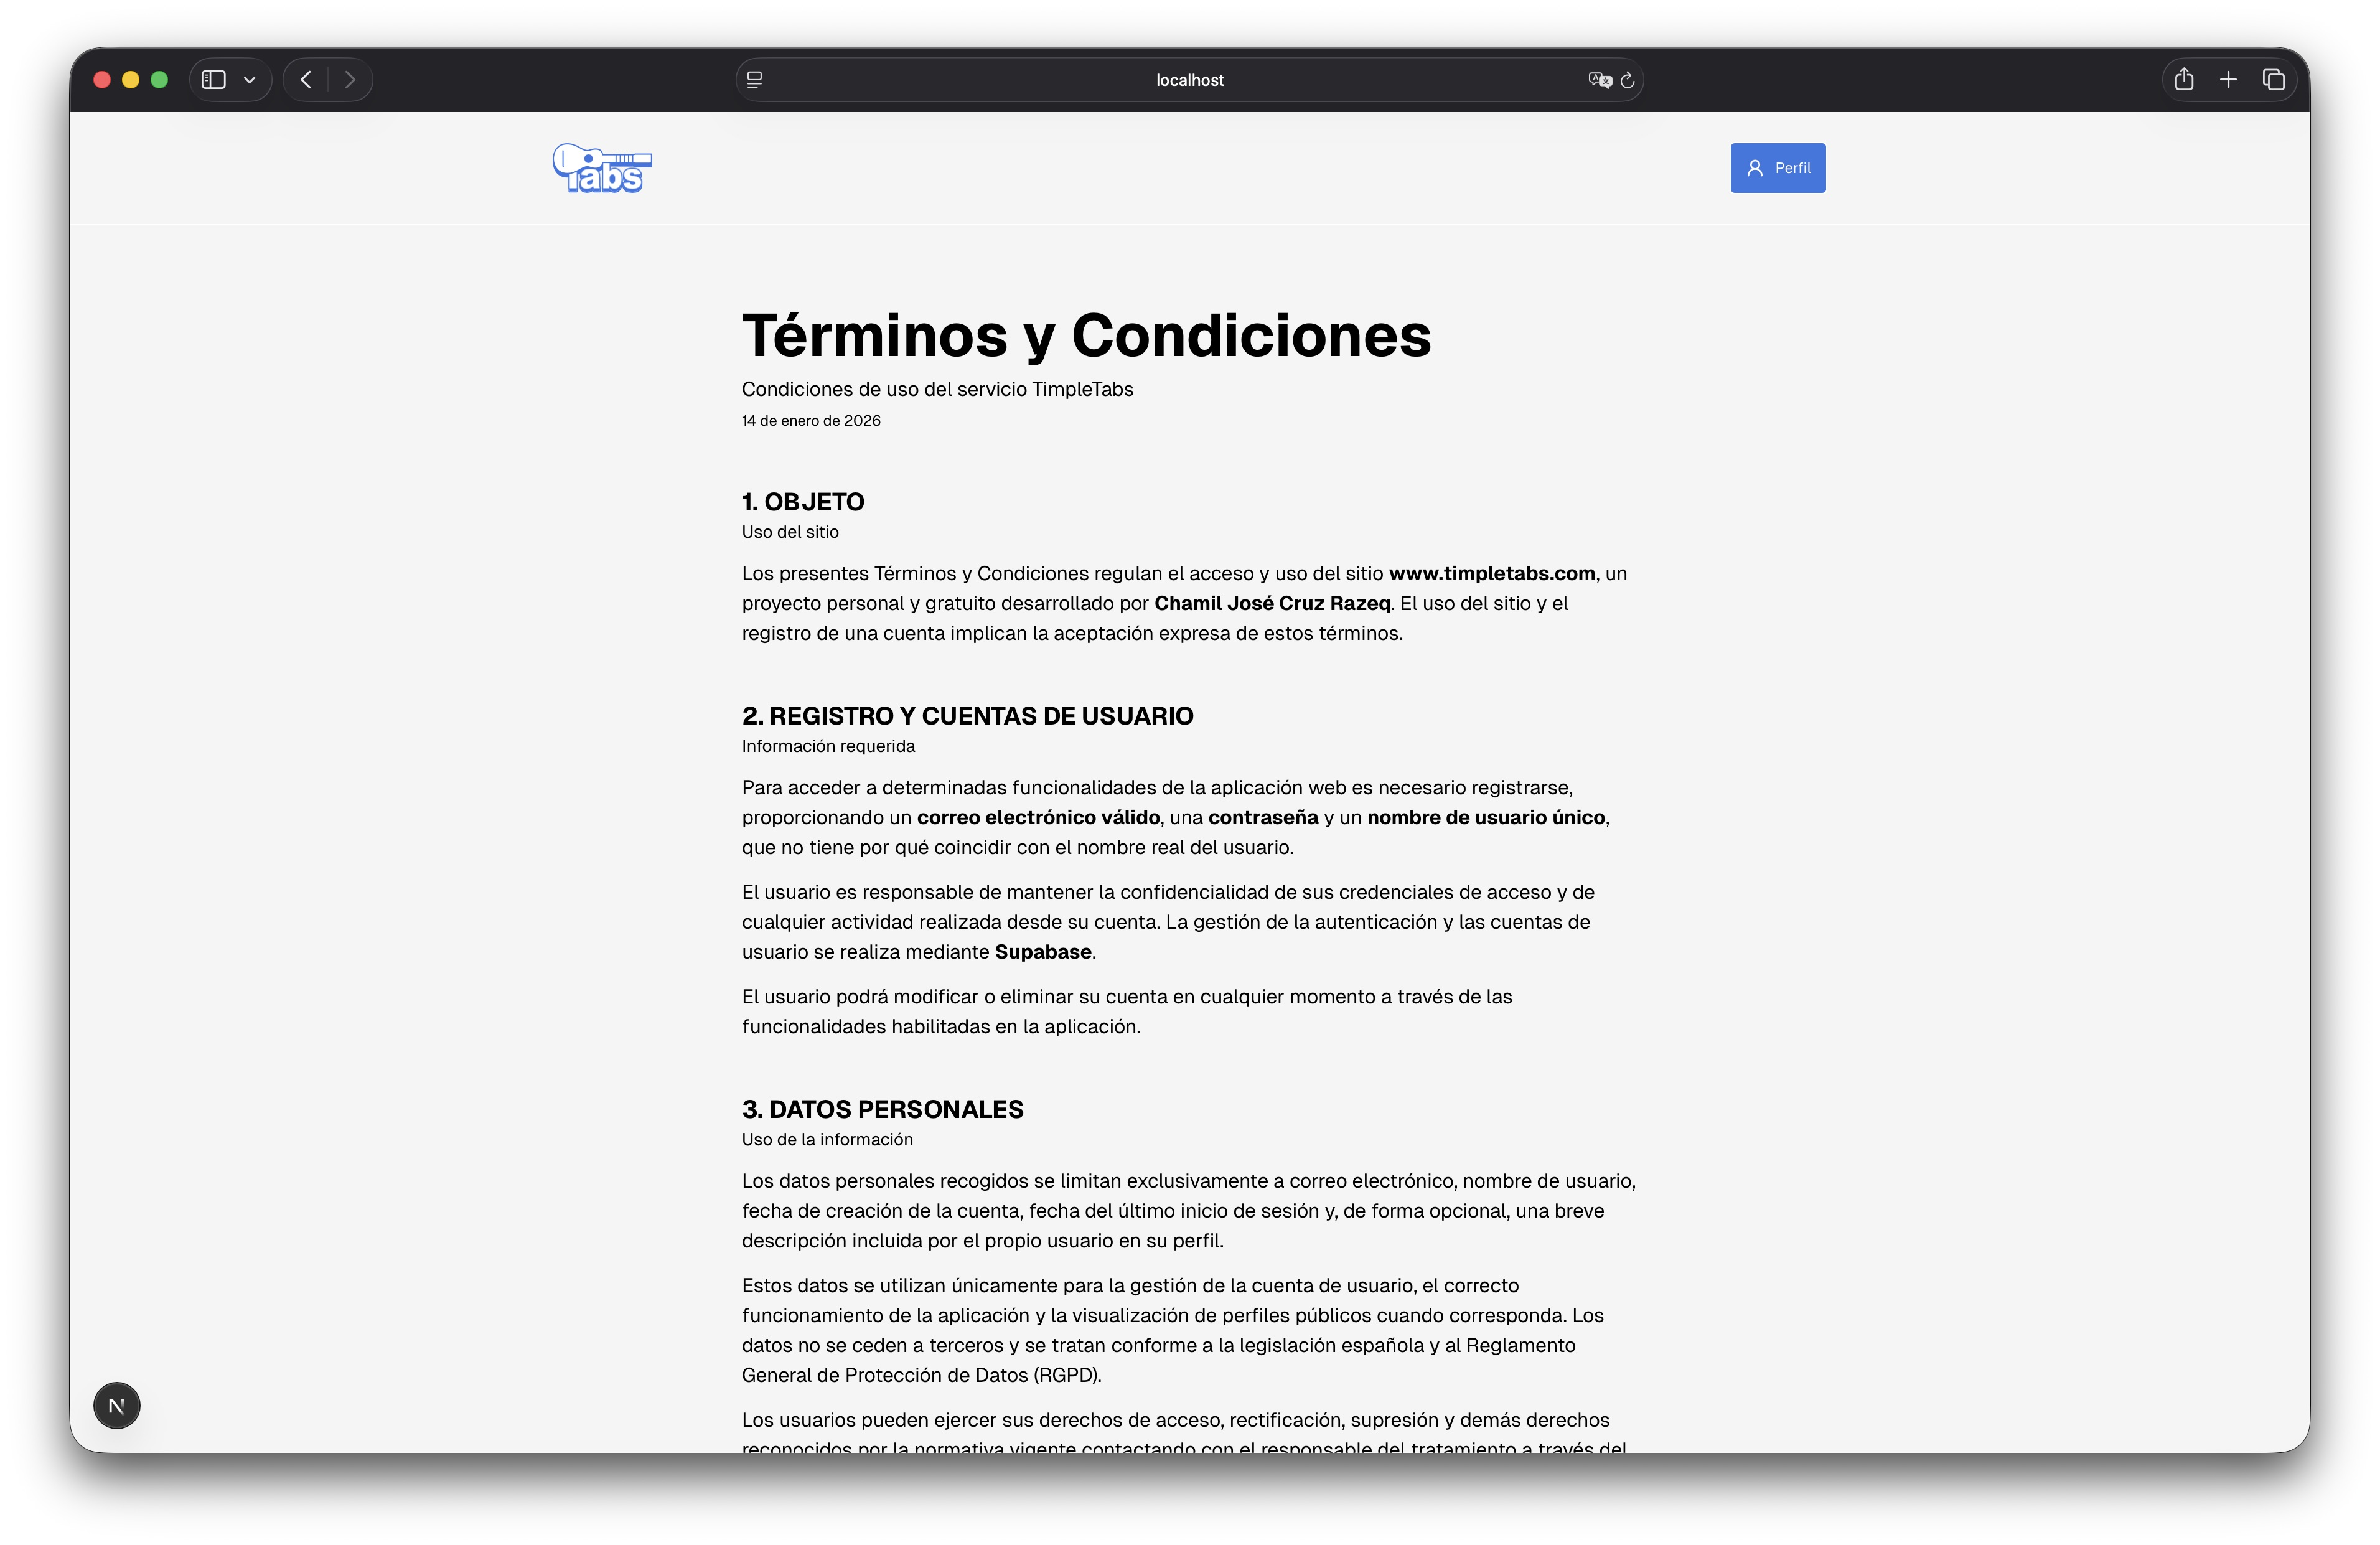
\includegraphics[width=0.8\textwidth]{Ilustraciones/desarrollo/incremento1/desarrollo/tac_it1.jpeg}
        \caption{Página de términos y condiciones del servicio}\label{fig:tac_it1}
    \end{figure}

\end{itemize}

\textbf{Finalmente}, se desarrollaron pruebas unitarias \figref{fig:tests_i1} por cada componente del lado del servidor, permitiendo verificar distintos comportamientos \textit{(i.e. manejo y propagación de errores, manejo y propagación de validaciones y casos favorables)}.

\begin{figure}[H]
    \centering
    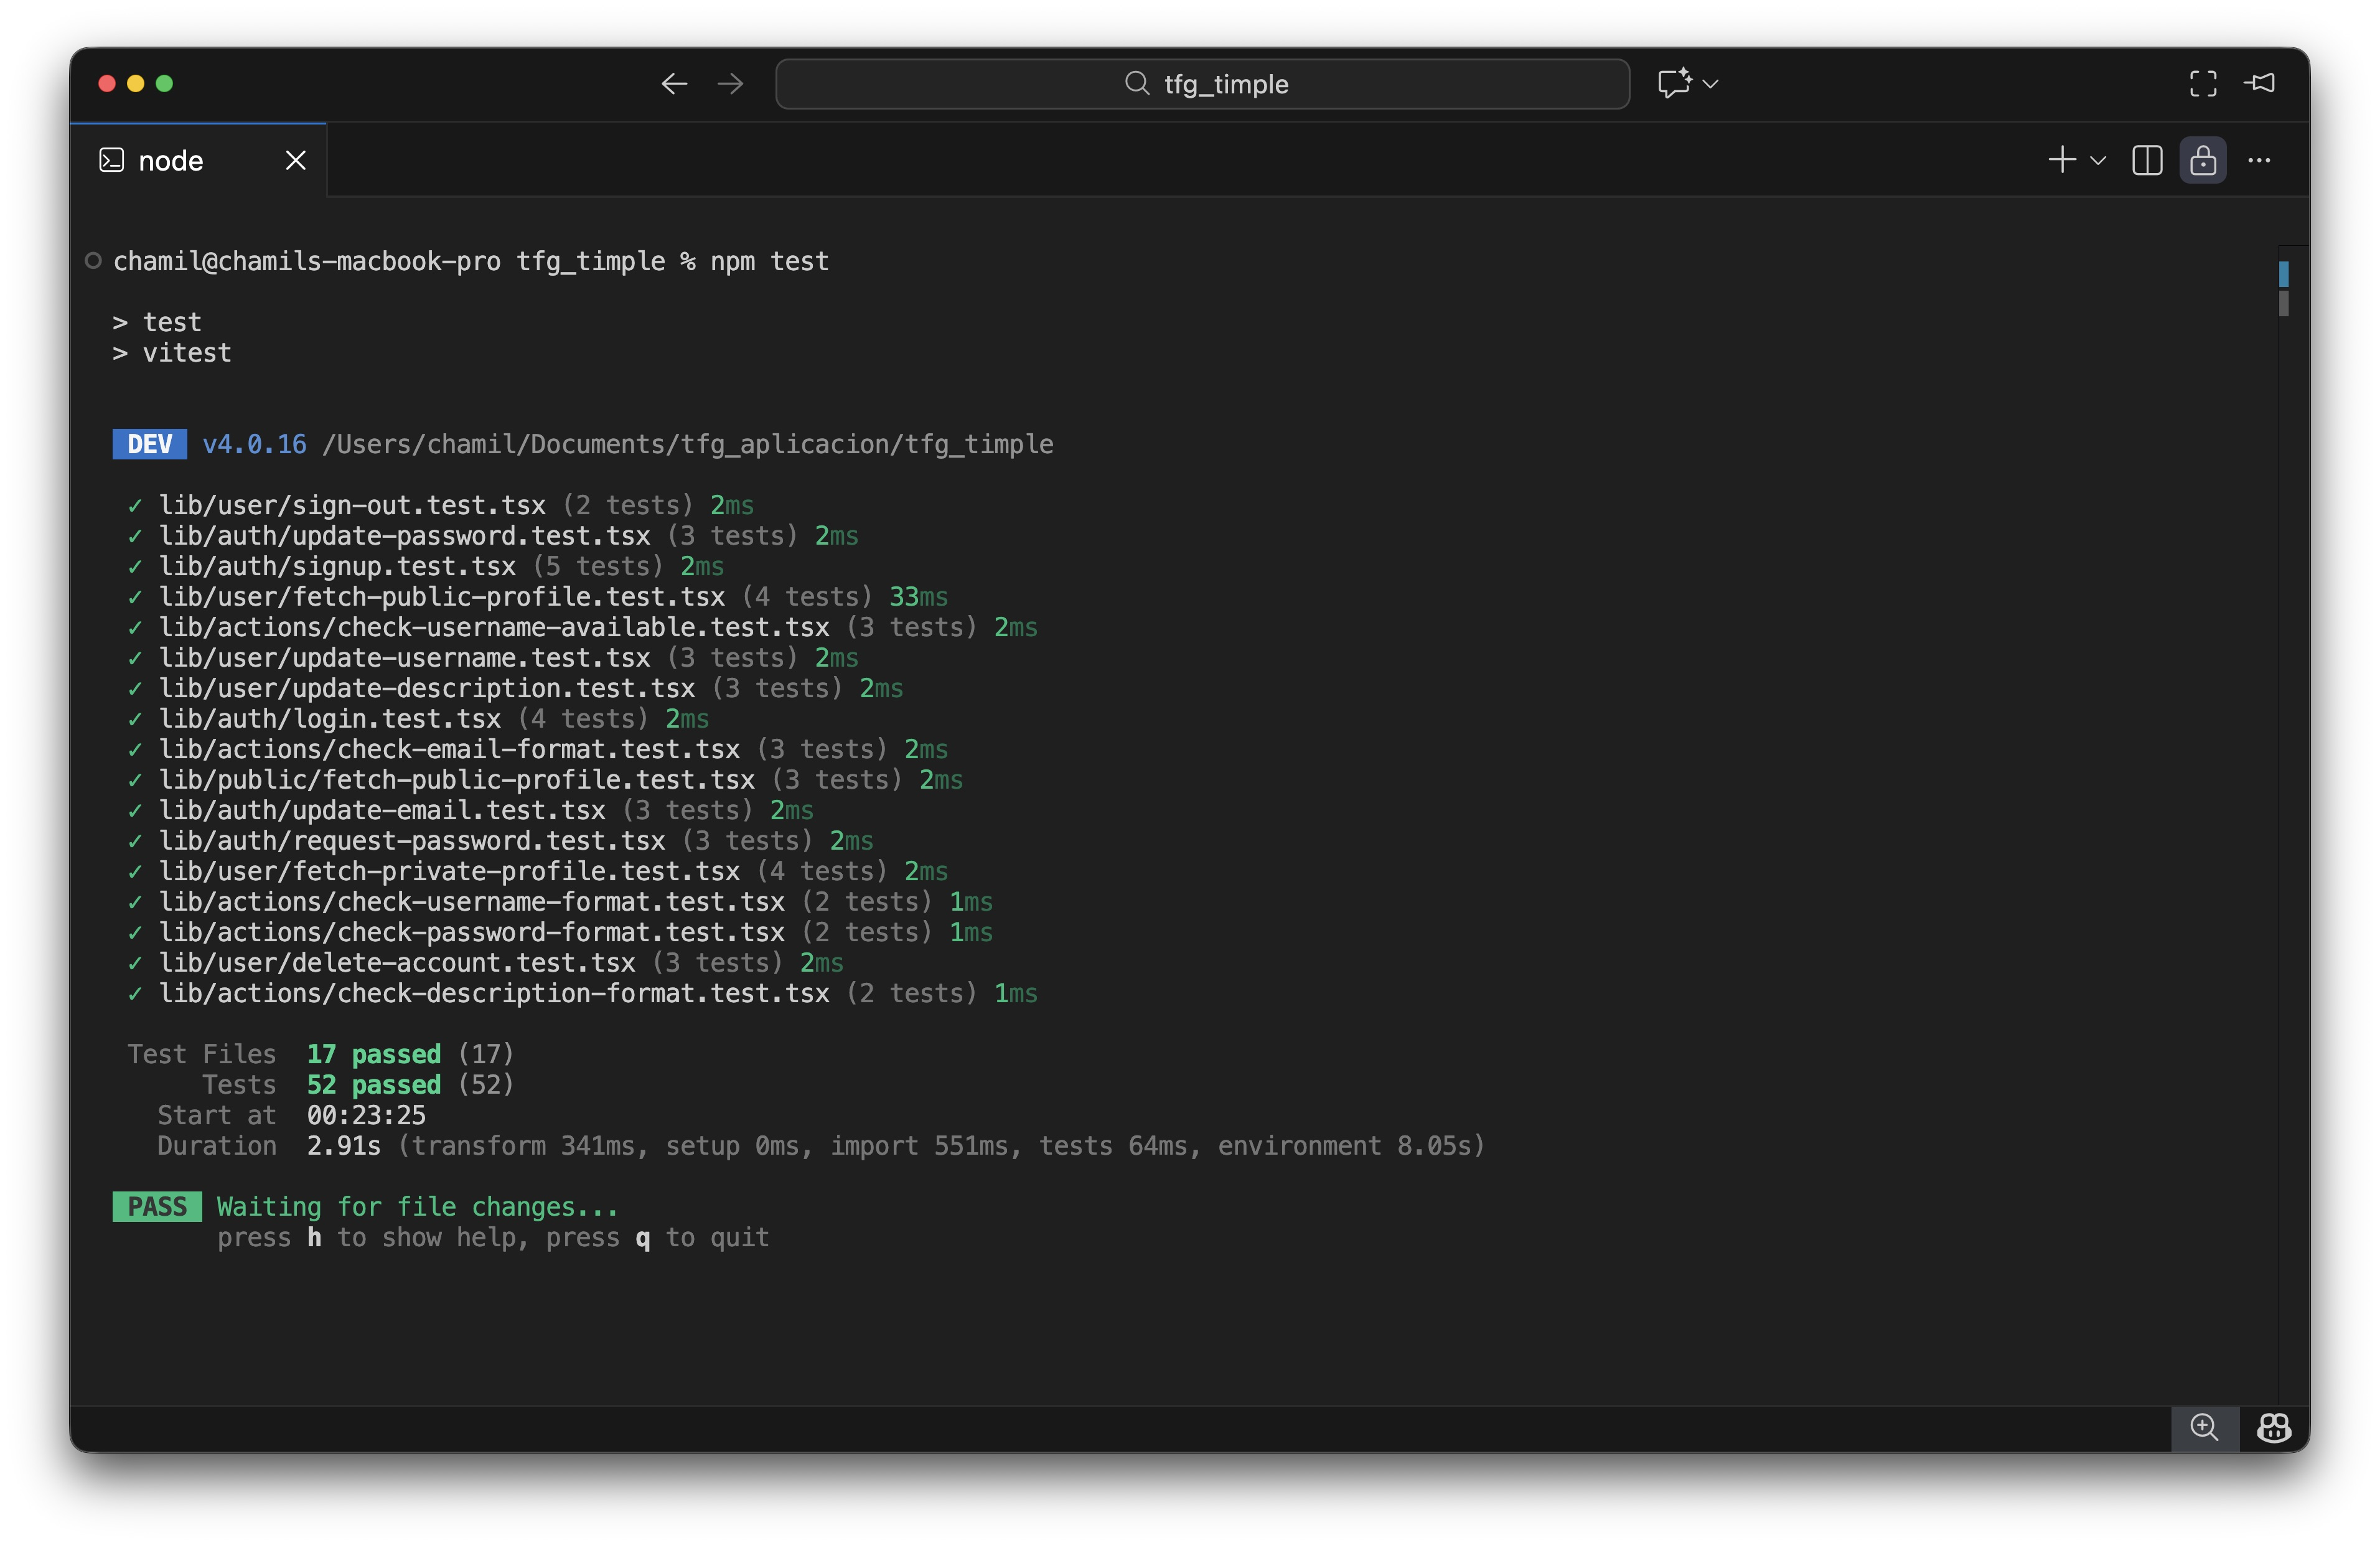
\includegraphics[width=0.8\textwidth]{Ilustraciones/desarrollo/incremento1/desarrollo/tests_i1.jpeg}
    \caption{Ejecución de pruebas del incremento 1 utilizando \textit{Vitest}}\label{fig:tests_i1}
\end{figure}

Además, se auditaron las páginas \figref{fig:lighthouse_i1}, evaluando aspectos de rendimiento, accesibilidad, SEO y buenas prácticas de desarrollo, obteniendo resultados satisfactorios.

\begin{figure}[H]
    \centering
    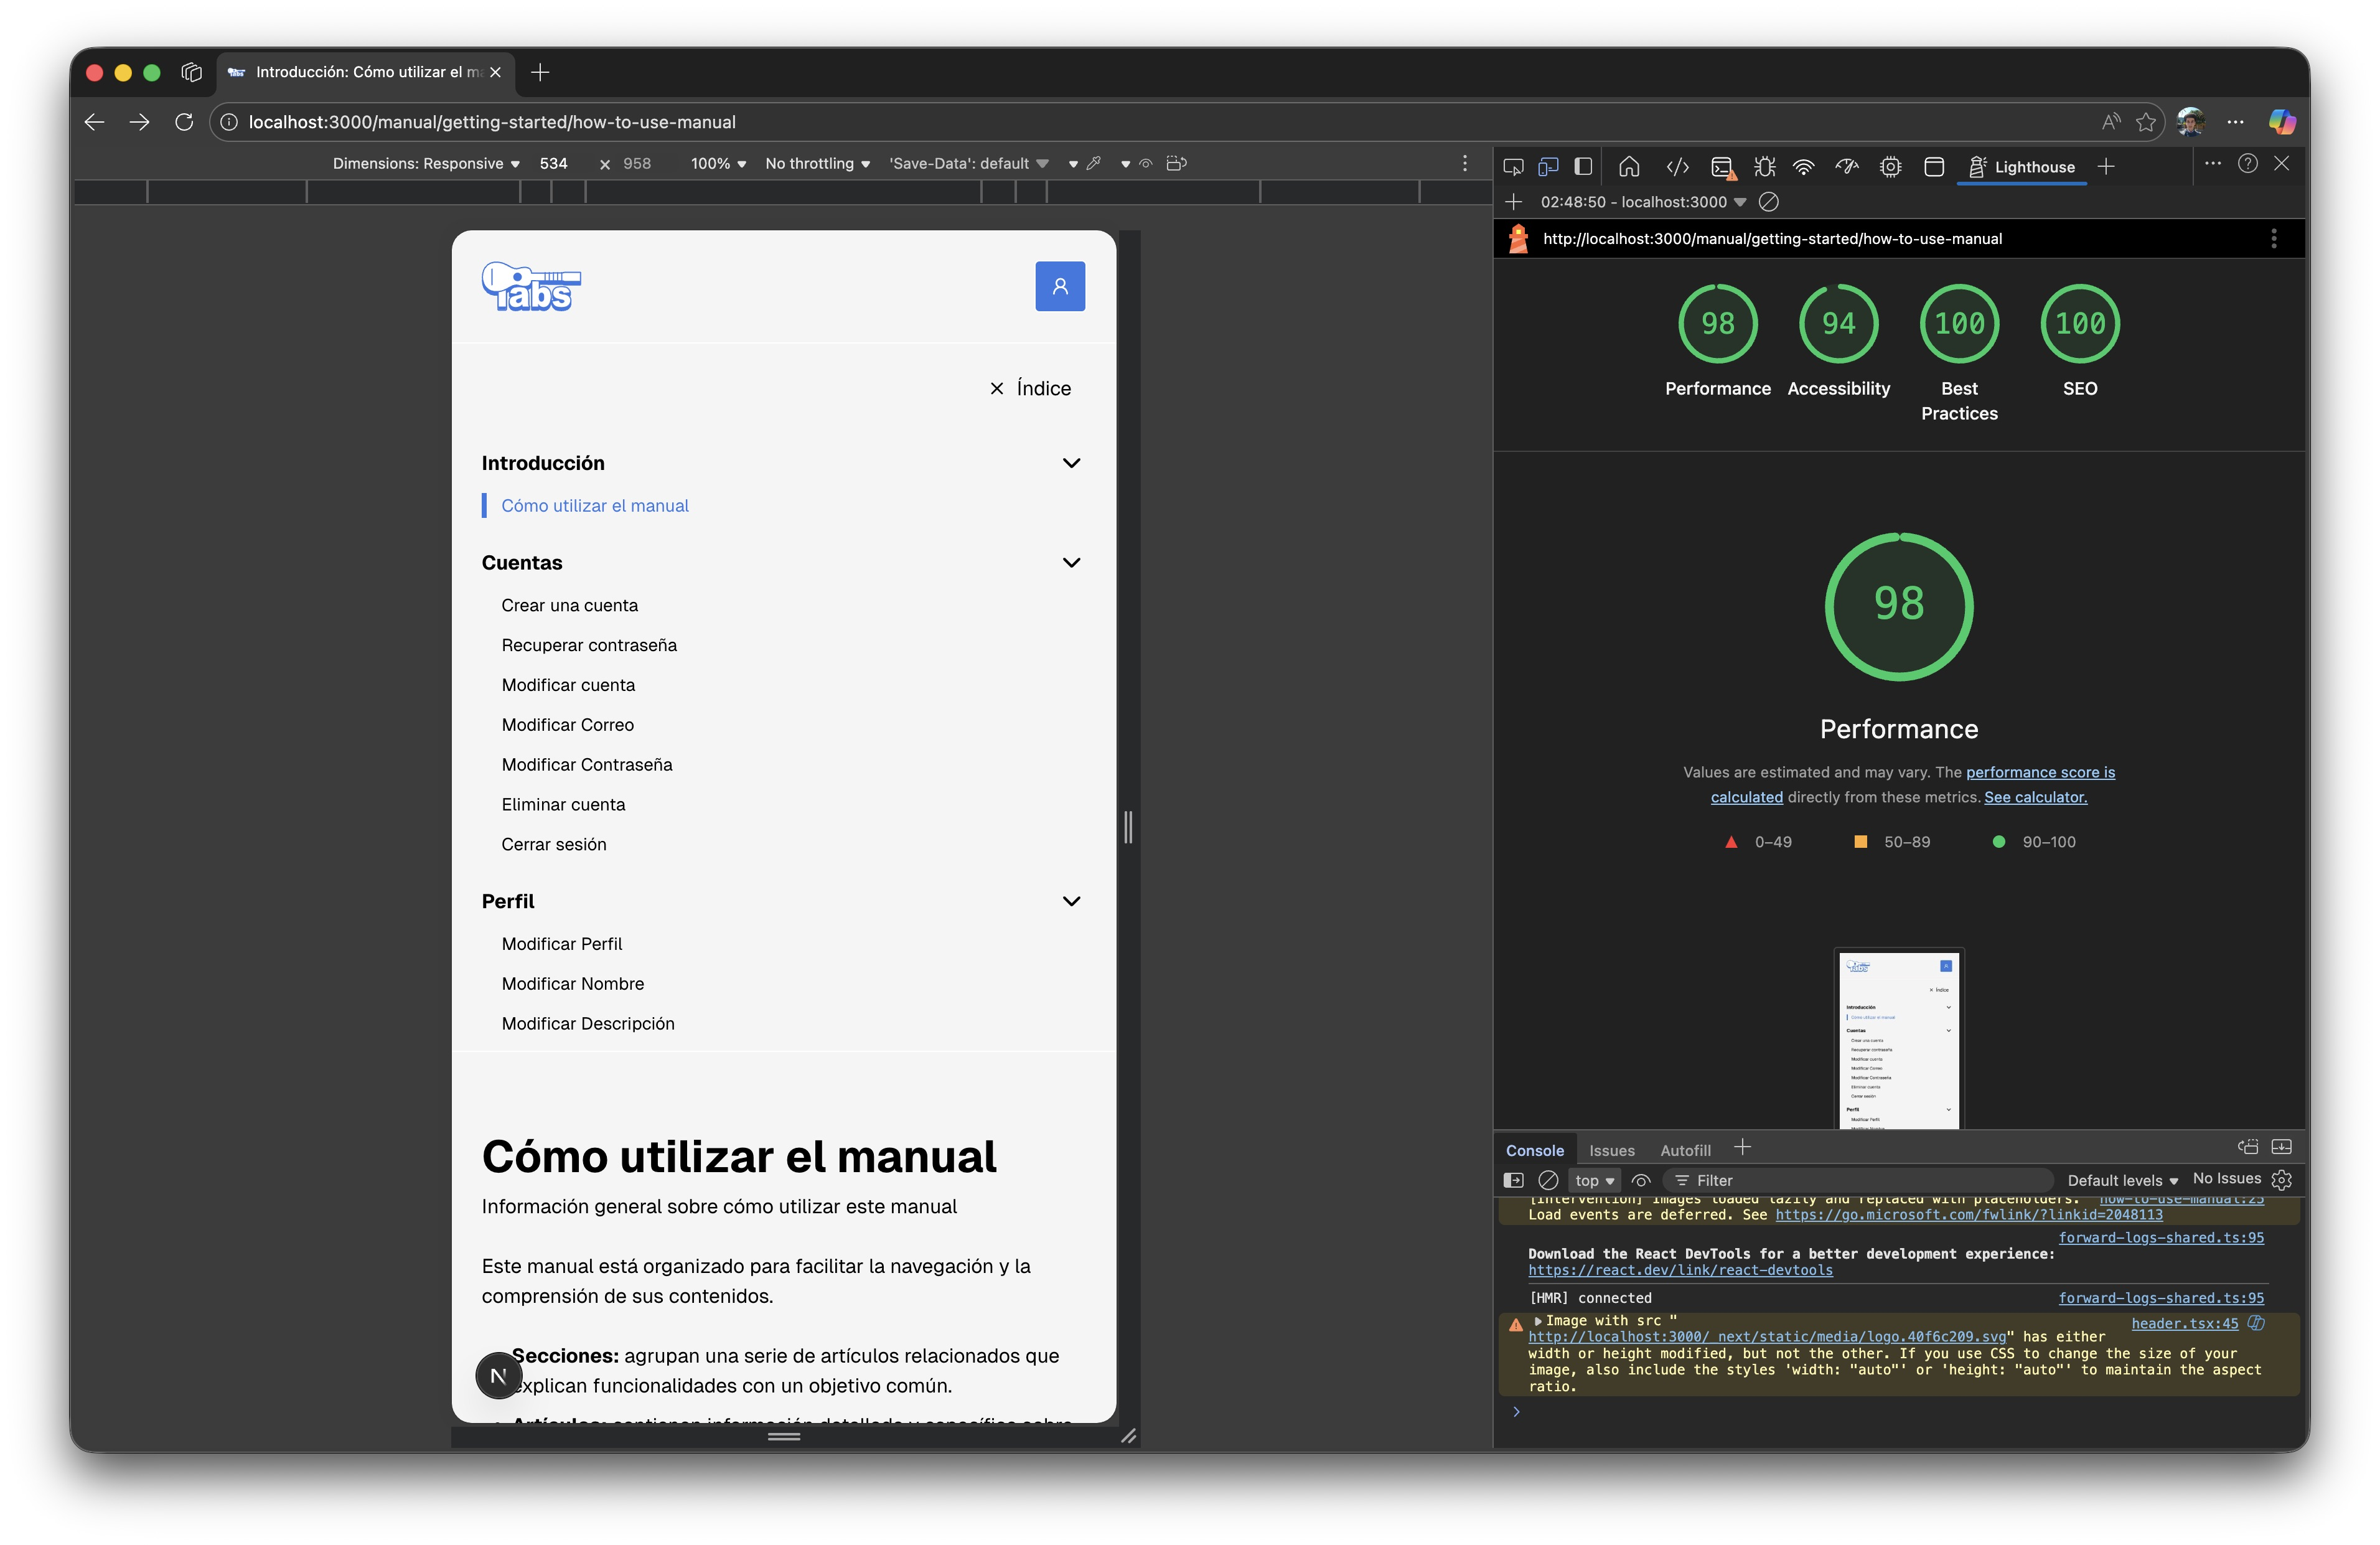
\includegraphics[width=0.8\textwidth]{Ilustraciones/desarrollo/incremento1/desarrollo/lighthouse_it1.jpeg}
    \caption{Resultados de auditoría del incremento 1 en \textit{Lighthouse}}\label{fig:lighthouse_i1}
\end{figure}
